\documentclass[11pt, spanish]{report}
\usepackage[spanish, activeacute]{babel}
\usepackage{amsmath}
\usepackage{graphicx}
\usepackage{url}

\begin{document}

\begin{titlepage}

  \begin{figure}[htp]
    \centering
    \mbox{
\includegraphics[scale=0.3]{cebolla.jpg}}
  \end{figure}
  
  \vspace*{2.0cm}
  \begin{center}
    {\Huge CNC\\} 
    {\LARGE Informe Entrega II\\}
    {\Large Lenguajes de Programaci\'on II \\ Abril - Julio 2010\\}
    \vspace{3.0cm}
    
    Federico Ponte - 06-40108\\
    Mar\'ia Gabriela Vald\'es - 05-39020\\
    
    \vspace*{2.0cm}
    Universidad Sim\'on Bol\'ivar.\\
    Caracas, Venezuela.\\
    \today
  \end{center}
  
\end{titlepage}

\newpage

\tableofcontents

\listoffigures

\newpage

\chapter{Introducci\'on}

Desde hace ya muchos a\~nos que se cre\'o la primera computadora. \'Esta fue creada en 1947 con el nombre de ENIAC (Electronic Numerical 
Integrator And Calculator). Desde ese d\'ia en adelante no han parado de aparecer nuevas computadoras cada vez m\'as peque\~nas y para 
diversos usos. Actualmente, las personas no se pueden imaginar un mundo sin \'estas y siempre que las usan se hacen la misma pregunta: 
c\'omo es que algo "inherte" tiene la capacidad entender las ordenes que se le dan y lograr cosas tan complejas.\\

\begin{figure}[htp]
  \centering
  \mbox{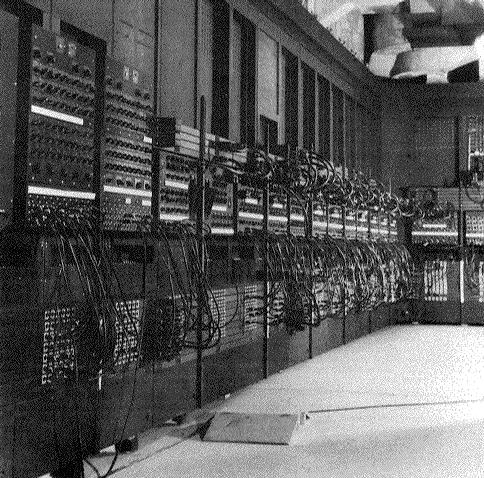
\includegraphics[scale=0.5]{eniac.jpg}}
  \caption{ENIAC}
  \label{fig eniac}
\end{figure}
  
Un modo f\'acil de responder ser\'ia el siguiente: las computadoras  lo \'unico que reconocen son 1's y 0's (hay o no hay voltaje), por lo 
que simplemente se le da una secuencia binaria con lo que uno desea que haga y listo. Pero que sucede si se quiere hacer un programa muy 
completo que requiera por lo menos de un mill\'on de n\'umeros binarios. Va a ser muy dif\'icil para un humano y se va a perder mucho 
tiempo haci\'endolo.\\

Para evitar este tipo de inconvenientes es que surge el estudio lenguajes de programaci\'on. La idea es poder tener un conjunto de frases 
capaces de expresar de un modo mucho m\'as simple lo mismo que los 1's y 0's que entiende una computadora. \'Estos pueden tener diferentes 
paradigmas: funcional, l\'ogico, imperativo, etc. As\'i como pueden ser interpretados o traducidos.\\

\section{Motivaci\'on del proyecto}

A medida que pasa el tiempo cada d\'ia surgen nuevos lenguajes: siempre se est\'a en la b\'usqueda de facilitarle las tareas al programador o 
cumplir ciertas tareas espec\'ificas. Lo que nunca se observa es el complejo trabajo que significa dise\~nar e implementar uno de \'estos.\\

Por ello la idea de este proyecto es justamente dise\~nar un lenguaje de tama\~no medio y crear un compilador para \'este.\\

Adem\'as uno como programador siempre tiene disgustos con algunas cosas de cada uno de los lenguajes.  As\'i, al crear un lenguaje propio 
con las cosas que a uno m\'as le agradan es bastante motivante.\\

\section{Breve descripci\'on del problema}

Como bien se mencion\'o antes el problema es ciertamente bastante complicado. El dise\~no de un lenguaje toma un tiempo considerable y largo, 
ya que se tiene que considerar una gran cantidad de aspectos. La idea es que \'este sea consistente y cumpla con su objetivo.\\

En cuanto a la implementaci\'on, \'esta se hace en varias faces. Primero se crea un analizador lexicogr\'afico o lexer, que va a reconocer 
todas las palabras reservadas para el lenguaje. Luego se crea un analizador sint\'ctico que se encarga de  verificar si un programa est\'a 
sint\'acticamente bien formado seg\'un los lineamientos de dise\~no del lenguaje. Despu\'es se proceden a hacer chequeos de tipo, tambi\'en 
seg\'un el dise\~no del lenguaje. Finalmente el \'arbol generado del analizador sint\'actico, es traducido a c\'odigo de m\'aquina para luego 
ser ejecutado.\\

\subsection{Palabras reservadas}

Las palabras reservadas de nuestro lenguaje y que no pueden ser utilizadas como identificadores son: 

\begin{verbatim}
int float bool char union struct break if elif else switch case 
default typedef for while const true false void return main read 
print
\end{verbatim}

Los siguientes caracteres tambien estan reservados como separadores del lenguajes: 

\begin{verbatim}
(  )  {  }  [  ]  ;  ,  .
\end{verbatim}

Los siguientes 19 tokens son operadores del lenguaje formados por los caracteres: 

\begin{verbatim}
=  ==  +  -  ++  --  *  /  %  !=  <  >  <=  >=  ||  &&  !  :  &
\end{verbatim}

Adem\'as tambi\'en est\'an reservados:

\begin{itemize}
\item N\'umeros literales.
\item Caracteres literales.
\end{itemize}

\subsection{Estructura general de un programa en CNC}

En el dise\~no del lenguaje se defini\'o que el orden estructural de un programa era el siguiente:

\begin{itemize}
\item Una secuencia de declaraciones de variables globales.
\item Una secuencia de promesas.
\item Una secuencia de declaraciones de funciones y procedimientos.
\item Pograma principal \emph{main}.
\end{itemize}

\section{Contenido del Informe}

El objetivo de este curso es desarrollar un lenguaje de programaci\'on y el prop\'osito de este informe es exponer los detalles de 
dise\~no de nuestro lenguaje, explicando m\'as espec\'ificamente el dise\~no de tipos b\'asicos y compuestos, instrucciones, funciones y procedimientos. 
En la secci\'on de implementaci\'on se mencionan las herramientas que utilizamos para el desarrollo del lenguaje, unido a la descripci\'on 
de los elementos m\'as importantes que fueron implementados, as\'i como la especificaci\'on de las clases que se construyeron y la estructura 
general de la gram\'atica. Tambi\'en en esta secci\'on se exponen los problemas que se nos presentaron durante las distintas etapas de 
desarrollo del lenguaje, as\'i como las soluciones propuestas e implementadas para resolver dichos conflictos. Seguido de este cap\'itulo 
se explican los detalles de compilaci\'on y corrida de la aplicaci\'on, para luego terminar con una rese\~na general del estado actual de 
nuestro proyecto y de los errores que no pudimos resolver.\\

\chapter{Dise\~no}
\section{Lineamientos}

El nombre de nuestro lenguaje es ``CNC" que quiere decir, ``C is not C". En lineas generales, el dise\~no del mismo est\'a basado en el dise\~no 
del lenguaje C. La raz\'on principal es que C es un lenguaje que tiene una sint\'axis sencilla pero que al mismo tiempo es muy poderoso y eficiente. 
\'Estas dos \'ultimas son caracter\'isticas favorables y ventajosas para un lenguaje y para los programadores que lo utilizan. Adem\'as buscamos 
que nuestro lenguaje sea un poco m\'as amigable que C en cuanto a la notificaci\'on y depuraci\'on de errores para el programador.\\

Este lenguaje es est\'aticamente tipeado. Los chequeos de tipos y declaraciones se hacen en tiempo de compilaci\'on. Por la misma raz\'on,
el lenguaje no permite reserva de memoria en tiempo de ejecuci\'on porque no se hace manejo de la memoria heap; s\'olo de la memoria est\'atica 
y de pila para los procedimientos, funciones y llamadas recursivas de los mismos.\\

\section{Operadores}
A continuaci\'on se numeran los operadores en orden de precedencia y se especifica su asociatividad:

\begin{itemize}
\item \begin{verbatim} - (unario), !, --, ++ \end{verbatim}
\item \begin{verbatim} *, /, % \end{verbatim}
\item \begin{verbatim} +, - \end{verbatim}
\item \begin{verbatim} <, <=, >, >= \end{verbatim}
\item \begin{verbatim} ==, != \end{verbatim}
\item \begin{verbatim} &&, || \end{verbatim}
\item \begin{verbatim} = \end{verbatim}
\end{itemize}

\begin{itemize}
\item Asociativos a la derecha: \begin{verbatim} = \end{verbatim}
\item Asociativos a la izquierda: \begin{verbatim} &&, ||, +, -, *, /, % \end{verbatim}
\item No asociativos: \begin{verbatim} ==, !=, <, <=, >, >=, - (unario), !, --, ++ \end{verbatim}
\end{itemize}

\section{Tipos B\'asicos}

\subsection{Int}
\begin{itemize}
\item \textbf{Declaraci\'on:}
  \begin{verbatim}
    int Identificador;
  \end{verbatim}
\item \textbf{Detalles:}
  Con este tipo de datos podr\'an representarse los n\'umeros enteros. \'Este ocupar\'a un tama\~no de 8 bytes en memoria.\\
\item \textbf{Operadores:}
  \begin{itemize}
    \item Los operadores de comparacion cuyo resultado es del tipo \emph{bool}: 
      \begin{itemize}
      \item Los operadores de comparacion num\'erica: \begin{verbatim} <, <=, >, >= \end{verbatim}
      \item Los operadores de equivalencia num\'erica: \begin{verbatim} ==, != \end{verbatim}
      \end{itemize}
    \item Los operadores num\'ericos cuyo resultado es del tipo \emph{int}:
      \begin{itemize}
        \item El operador de menos unario: \begin{verbatim} - \end{verbatim}
        \item Los operadores aditivos: \begin{verbatim} +, - \end{verbatim}
        \item Los operadores de multiplicativos: \begin{verbatim} *, /, % \end{verbatim}
        \item Los operadores de incremento (s\'olo se permite con identificadores): \begin{verbatim} ++, -- \end{verbatim}
      \end{itemize}
    \item El operador de asignaci\'on:
        \begin{verbatim} = \end{verbatim}
        Cuyo resultado es el mismo valor que se est\'a asignando, luego de haber hecho las conversiones impl\'icitas necesarias.
  \end{itemize}
\end{itemize}

\subsection{Float}

\begin{itemize}
\item \textbf{Declaraci\'on:}
  \begin{verbatim}
    float Identificador;
  \end{verbatim}
\item \textbf{Detalles:}
  Con este tipo de datos podr\'an representarse los n\'umeros reales. Los \emph{float} ocupar\'an un tama\~no de 8 bytes en memoria.\\
\item \textbf{Operadores:}
  \begin{itemize}
  \item Los operadores de comparacion cuyo resultado es del tipo \emph{bool}: 
    \begin{itemize}
    \item Los operadores de comparacion num\'erica: \begin{verbatim} <, <=, >, >= \end{verbatim}
    \item Los operadores de equivalencia num\'erica: \begin{verbatim} ==, != \end{verbatim}
    \end{itemize}
  \item Los operadores num\'ericos cuyo resultado es del tipo \emph{float}:
    \begin{itemize}
    \item El operador de menos unario: \begin{verbatim} - \end{verbatim}
    \item Los operadores aditivos: \begin{verbatim} +, - \end{verbatim}
    \item Los operadores de multiplicativos: \begin{verbatim} *, / \end{verbatim}
    \item Los operadores de incremento(s\'olo se permite con identificadores): \begin{verbatim} ++, -- \end{verbatim}
    \end{itemize}
  \item El operador de asignaci\'on:
    \begin{verbatim} = \end{verbatim}
    Cuyo resultado es el mismo valor que se est\'a asignando, luego de haber hecho las conversiones impl\'icitas necesarias.
  \end{itemize}
\end{itemize}

\subsection{Char}
\begin{itemize}
\item \textbf{Declaraci\'on:}
  \begin{verbatim}
    char Identificador;
  \end{verbatim}
\item \textbf{Detalles:}
  Los caracteres ocupar\'an 8 bytes en memoria. \'Estos ser\'an \'utiles junto con el tipo de dato \emph{Array}, para poder simular el 
  tipo de dato "String" que nuestro lenguaje no posee expl\'icitamente.\\

  Es importante justificar que decidimos que los caracteres ocupar\'ian 8 bytes a bajo nivel, para hacer m\'as f\'acil el manejo de los bits
  en memoria ya que la memoria est\'a alineada siempre y los registros que utilizamos son todos de tama\~no de 64-bits. \'Esto evita
  el uso de máscaras y desplazamientos para obtener un valor.\\

  En cuanto a los operadores de comparaci\'on estos simplemente van a usar el valor ascii. Es decir, si se compara 'a'>'b', \'esto devuelve falso
  ya que el c\'odigo ascii de 'a' es 97 y el de 'b' 98.\\

\item \textbf{Operadores:}
  \begin{itemize}
  \item Los operadores de comparacion cuyo resultado es del tipo \emph{bool}: 
    \begin{itemize}
    \item Los operadores de comparacion: \begin{verbatim} <, <=, >, >= \end{verbatim}
    \item Los operadores de equivalencia: \begin{verbatim} ==, != \end{verbatim}
    \end{itemize}
  \item Los operadores num\'ericos cuyo resultado es del tipo \emph{char}:
    \begin{itemize}
    \item Los operadores de incremento(s\'olo se permite con identificadores): \begin{verbatim} ++, -- \end{verbatim}
    \end{itemize}
  \item El operador de asignaci\'on:
    \begin{verbatim} = \end{verbatim}
    Cuyo resultado es el mismo valor que se est\'a asignando, luego de haber hecho las conversiones impl\'icitas necesarias.
  \end{itemize}
\end{itemize}

\subsection{Bool}
\begin{itemize}
\item \textbf{Declaraci\'on:}
  \begin{verbatim}
    bool Identificador;
  \end{verbatim}
\item \textbf{Detalles:}
  El tipo de dato \emph{bool} ocupar\'an 8 bytes en memoria, al igual que los caracteres. Cabe destacar que las expresiones booleanas son las que
  determinan el control de flujo de las siguientes instrucciones: \begin{verbatim} if, while, for \end{verbatim}.\\

  Al igual que con los caracteres, los booleanos van a ocupar 8 bytes a bajo nivel por el mismo motivo de hacer m\'as f\'acil el manejo de los bits
  en memoria a la hora de generar c\'odigo ya que la memoria est\'a alineada siempre.\\

\item \textbf{Operadores:}
  \begin{itemize}
  \item Los operadores relacionales: \begin{verbatim} ==, != \end{verbatim}
  \item El operador de complemento l\'ogico: \begin{verbatim} ! \end{verbatim}
  \item Los operadores l\'ogicos: \begin{verbatim} &&, || \end{verbatim}
  \item El operador de asignaci\'on:
    \begin{verbatim} = \end{verbatim}
    Cuyo resultado es el mismo valor que se est\'a asignando, luego de haber hecho las conversiones impl\'icitas necesarias.
  \end{itemize}
\end{itemize}

\section{Conversi\'on de Tipos B\'asicos}
Cuando se realizan operaciones entre tipos b\'asicos distintos, la conversi\'on se hace impl\'icitamente seg\'un la siguiente tabla de cohersi\'on, donde N/A se refiere a que la conversi\'on entre dichos tipos ``No Aplica'', y por el contrario A significa que ``Aplica'':\\

Para los operadores aritm\'eticos: 

\begin{verbatim} 
+, -, *, /, % 
\end{verbatim}

\begin{table}[!hbp]
  \begin{tabular}{c c c c c}
    \hline            
    Tipo  & int   & float & bool & char \\ [0.5ex]
    \hline                         
    int   & int   & float & N/A  & N/A \\        
    float & float & float & N/A  & N/A \\
    bool  & N/A   & N/A   & N/A  & N/A \\
    char  & N/A   & N/A   & N/A  & N/A \\ [1ex]
    \hline
  \end{tabular}    
\end{table}
  
Para los operadores de comparaci\'on:

\begin{verbatim} 
==, !=
\end{verbatim}

\begin{table}[!hbp]
  \begin{tabular}{c c c c c}
    \hline            
    Tipo  & int & float & bool & char \\ [0.5ex]
    \hline                         
    int   & A   & A     & N/A  & A \\        
    float & A   & A     & N/A  & N/A \\
    bool  & N/A & N/A   & A    & N/A \\
    char  & A   & N/A   & N/A  & A \\ [1ex]
    \hline                         
  \end{tabular}    
\end{table}

\begin{verbatim} 
<, <=, >, >= 
\end{verbatim}

\begin{table}[!hbp]
  \begin{tabular}{c c c c c}
    \hline            
    Tipo  & int & float & bool & char \\ [0.5ex]
    \hline                         
    int   & A   & A     & N/A  & A \\        
    float & A   & A     & N/A  & N/A \\
    bool  & N/A & N/A   & N/A  & N/A \\
    char  & A   & N/A   & N/A  & A \\ [1ex]
    \hline                         
  \end{tabular}    
\end{table}

\newpage

Para los operadores booleanos:

\begin{verbatim} 
&&, ||
\end{verbatim}

\begin{table}[!hbp]
  \begin{tabular}{c c c c c}
    \hline            
    Tipo  & int & float & bool & char \\ [0.5ex]
    \hline                         
    int   & N/A & N/A   & N/A  & N/A \\        
    float & N/A & N/A   & N/A  & N/A \\
    bool  & N/A & N/A   & A    & N/A \\
    char  & N/A & N/A   & N/A  & N/A \\ [1ex]
    \hline                         
  \end{tabular}    
\end{table}

En este caso se indica el tipo resultante de asignar fila con columna. Para el operador de asignaci\'on, y los par\'ametros de llamadas a subrutinas: 

\begin{table}[!hbp]
  \begin{tabular}{c c c c c}
    \hline            
    Tipo  & int   & float & bool & char \\ [0.5ex]
    \hline                         
    int   & int   & int & N/A    & N/A \\        
    float & float & float & N/A  & N/A \\
    bool  & N/A   & N/A   & bool & N/A \\
    char  & char  & N/A   & N/A  & char \\ [1ex]
    \hline
  \end{tabular}    
\end{table}

La conversión de flotante a entero truncando el valor entero del flotante. En \'este caso se pierde informaci\'on.

\subsection{Regla General}

  \begin{itemize}
  \item \textbf{int:} Son compatibles con los ellos mismos, flotantes y caracteres.
  \item \textbf{float:} Son compatibles con los ellos mismos y enteros.
  \item \textbf{bool:} S\'olo son compatibles con ellos mismos.
  \item \textbf{char:} Son compatibles con ellos mismos y los enteros.
  \end{itemize}

  Todo \'esto siguiendo las reglas antes descritas.


\section{Tipos Compuestos}

\subsection{Arreglos}
\begin{itemize}
\item \textbf{Declaraci\'on:}
  \begin{verbatim}
    Tipo [Constante entera]...[Constante entera] Identificador;
  \end{verbatim}
\item \textbf{Detalles:}
  Cada [Constante entera] representa una dimensi\'on del arreglo y la expresi\'on indica su tama\~no. Adem\'as es importante mencionar que \emph{tipo} puede ser cualquier tipo b\'asico antes especificado, as\'i como un registro o uni\'on que se explicar\'an a continuaci\'on.\\
  
  En cuanto al almacenamiento en memoria, este tipo de dato se va alamcenar por filas, es decir, se recorre el arreglo de izquierda a derecha y de 
  arriba a abajo, y de este modo se almacenan, al igual que en el lenguaje C.\\

\item \textbf{Operadores:}
  \begin{itemize}
  \item El operador de asignaci\'on:
    \begin{verbatim} = \end{verbatim}
    Ser\'a v\'alido siempre y cuando las dimensiones y el tipo base de los arreglos involucrados en la operaci\'on sean asignables entre s\'i. Es 
    decir que si se tiene un arregle de flotantes y \'este se asigna a un arreglo de enteros, lo que se va a hacer es ir moviendo casilla por casilla
    del primer arreglo al segundo haciendo los cast de flotante a entero.
  \end{itemize}
\item \textbf{Inicializaci\'on:}
  \begin{verbatim}
    Tipo [Constante entera1]...[Constante enteran] Identificador = 
    { { {x, y, ... };  {p, q, ... }; ... }; ... ; { {z, w, ...}; ... } };
  \end{verbatim}

  Donde la lista exterior contiene tantos elementos, a su vez listas, como indique la Constante entera1, as\'i, cada una de estas listas ser\'a de tama\~no igual a la Constante entera2, y as\'i sucesivamente. Además x,y,p,q,z y w son expresiones.
\item \textbf{Acceso:}
  Para acceder a cierta pocisi\'on del arreglo, la notaci\'on que debe seguirse es la siguiente:
  \begin{verbatim}
    Identificador[Expresion1]...[Expresionn];
  \end{verbatim}

  Donde cada Expresi\'on\_i debe ser de tipo \emph{Int} con valores v\'alidos entre 0 y \emph{n} - 1, donde \emph{n} es el tama\~no de la dimensi\'on a la que le corresponden dichos corchetes.
\end{itemize}

\subsection{Registro}
\begin{itemize}
\item \textbf{Sint\'axis:}
  \begin{verbatim}
    struct {
      Tipo1 Identificador1;
      Tipo2 Identificador2;
      ...
      Tipon Identificadorn;
    } Identificador;
  \end{verbatim}
\item \textbf{Detalles:}
  Los registros son estructuras cuyo cuerpo lo conforman tipos b\'asicos o compuestos. Cada ``atributo'' de la estructura viene especificado con su tipo y 
  nombre correspondiente. Es importante recalcar que todos los identificadores dentro de la estructura deben ser diferentes entre si.\\

  El almacenamiento en memoria ser\'a como un bloque sin compactaci\'on, es decir, si se tiene:

  \begin{verbatim}
    struct { 
      bool a; 
      int b; 
    } x; 
  \end{verbatim}

  Esta estructura se almacenar\'ia as\'i:\\

  \begin{figure}[!htp]
    \centering
    \mbox{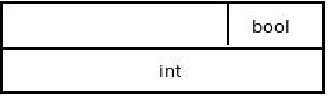
\includegraphics[scale=0.5]{memoria1.jpg}}
    \caption{Tipo de almacenamiento}
    \label{fig memoria1}
  \end{figure}

%\newpage
  y no as\'i:

  \begin{figure}[!htp]
    \centering
    \mbox{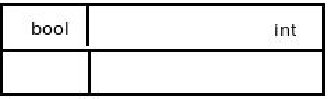
\includegraphics[scale=0.5]{memoria2.jpg}}
    \caption{Tipo de almacenamiento}
    \label{fig memoria2}
  \end{figure}
  
  Claro \'esta que en este ejemplo no va de acuerdo al lenguaje ya que los booleanos van a ocupar 8 bytes. Simplemente la idea era reflejar lo que es 
  compactaci\'on.
  Se escogi\'o este tipo de almacenamiento porque a pesar de que se pierde memoria, se gana eficiencia en el programa.\\

\item \textbf{Operadores:}
  \begin{itemize}
  \item El operador de asignaci\'on:
    \begin{verbatim} = \end{verbatim}
    Ser\'a v\'alido siempre y cuando la cantidad de campos, el orden de los mismos, los identificadores y el tipo asociado a cada uno de ellos, sean iguales en ambos de los registros involucrados en la operaci\'on. 
  \end{itemize}
\item \textbf{Inicializaci\'on:}
  \begin{verbatim}
    struct {
      Tipo1 Identificador1;
      Tipo2 Identificador2;
      ...
      Tipon Identificadorn;
    } Identificador = 
    {Identificador1 = Valor1; ... ; Identificadorn = Valorn} ;
  \end{verbatim}
\item \textbf{Acceso:}
  Para acceder a cierto campo del registro, la notaci\'on que debe seguirse es la siguiente:
  \begin{verbatim}
    Identificador.Campo_i;
  \end{verbatim}

  Donde Campo\_i, debe ser uno de los Identificadores\_i especificados en la declaraci\'on.
\end{itemize}

\subsection{Uni\'on}
\begin{itemize}
\item \textbf{Sint\'axis:}
  \begin{verbatim}
    union {
      Tipo1 Identificador1;
      Tipo2 Identificador2;
      ...
      Tipon Identificadorn;
    } Identificador;
  \end{verbatim}
\item \textbf{Detalles:}
  La sint\'axis de las uniones es igual a la de los registros. Lo que diferencia a las uniones de los registros es que \'estas s\'olo pueden tener 
  un campo activo de entre todos los que se especificaron en su declaraci\'on, \'este se actualiza y cambia a trav\'es de la operaci\'on de asignaci\'on. \\

  Para las uniones tambi\'en se cumple que su cuerpo lo conforman tipos b\'asicos o compuestos. Cada ``atributo'' de la estructura viene especificado 
  con su tipo y nombre correspondiente. Es importante recalcar que todos los identificadores dentro de la estructura deben ser diferentes entre si.\\

  La representaci\'on en memoria de este tipo complejo sigue el siguiente esquema:

  \begin{figure}[htp]
    \centering
    \mbox{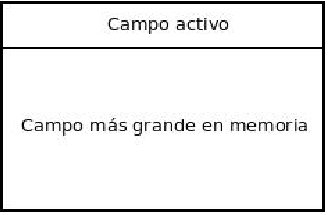
\includegraphics[scale=0.5]{memoria3.jpg}}
    \caption{Tipo de almacenamiento de las uniones}
    \label{fig memoria3}
  \end{figure}

  Con el almacenamiento del campo activo en memoria lo que se busca es evitar errores de asignaci\'on: asignar dos uniones con el campo activo diferente o también asignar a un campo activo que en verdad no lo est\'a. Por otro lado, como las uniones s\'olo poseen 
  un campo activo a la vez, basta con reservar espacio en memoria igual al campo de mayor tama\~no.\\
  
\item \textbf{Operadores:}
  \begin{itemize}
  \item El operador de asignaci\'on: 
    \begin{verbatim} = \end{verbatim}
    Ser\'a v\'alido siempre y cuando la cantidad de campos, el orden de los mismos (en el caso que se asigne una union con otra), los identificadores y el tipo asociado a cada uno de ellos, sean asignables en ambas de las uniones involucrados en la operaci\'on. Si se usa un literal de unión, el campo que se especifique en la asignaci\'on, ser\'a el campo activo de la uni\'on.\\

    \begin{verbatim}
      Identificador = {Campo_i = Valor_i} ;
    \end{verbatim}

  \item El operador de hasactive: 
    \begin{verbatim} hasactive \end{verbatim}
    La idea de este operador es permitir al programador en tiempo de ejecuci\'on saber si la uni\'on tiene el campo dado activo. \'Este devuelve
un booleano. Su uso es de la siguinte forma:\\

    \begin{verbatim}
      Union hasactive Campo
    \end{verbatim}

   Donde la el primer operando es el identificador de la uni\'on y el segundo un identificador con el campo que se quiere saber si se encuentra activo.
Un ejemplo real de uso seria el siguiente:

    \begin{verbatim}
      union{
         int a;
         bool b;
      } unionC;

      ...

      if(unionC hasactive b){
        ...
      }
      else{
        ...
      }
    \end{verbatim}


  \end{itemize}
\item \textbf{Inicializaci\'on:}
  \begin{verbatim}
    union {
      Tipo1 Identificador1;
      Tipo2 Identificador2;
      ...
      Tipon Identificadorn;
    } Identificador = {Campo_i = Valor_i} ;
  \end{verbatim}
\item \textbf{Acceso:}
  Para acceder a cierto campo de la uni\'on, la notaci\'on que debe seguirse es la siguiente:
  \begin{verbatim}
    Identificador.Campo_i;
  \end{verbatim}

  Donde Campo\_i, debe ser uno de los Identificadores\_i especificados en la declaraci\'on y adem\'as debe ser el campo activo, sino es un error.
\end{itemize}

\section{Instrucciones}

El conjunto de instrucciones que se tiene es el mismo que el de la mayor\'ia de los lenguajes imperativos modernos. Se us\'o la misma sint\'axis que C, C++ 
y Java con el objetivo de facilitar el aprendizaje del lenguaje. Adem\'as \'estas proporcionan suficiente poder de expresi\'on por lo que no se 
agreg\'o alguna instrucci\'on fuera de lo com\'un.\\

\subsection{Declaraciones}

\begin{itemize}
\item \textbf{Sint\'axis:}

  \begin{verbatim} 
    tipo Identificador;
    tipo Identificador, ..., Identificador;
    tipo Identificador = Expresion;
    tipo Identificador, ..., Identificador = Expresion;
  \end{verbatim} 

\item \textbf{Detalles:}
  La declaraci\'on es igual que en la mayor\'ia de lenguajes. Se puede hacer una declaraci\'on con o sin inicializaci\'on. En el caso que no se inicialicen, no se tienen valores por defecto. Se debe revisar que las variables esten inicializadas a la hora de usarlas. En el tercer y cuarto caso se 
  asigna el mismo valor de la expresi\'on a cada uno de los valores declarados.\\
  
  Un detalle importante de las declaraciones, es que \'estas se pueden hacer en los bloques de los \emph{if}, \emph{for}, \emph{switch} y \emph{while}. 
  En estos casos las variables s\'olo van a existir y van a tener alcance en la ejecuci\'on de dicho bloque. \\
  
  Cabe destacar, que no permitimos declaraciones anidadas de variables con igual identificador dentro de los bloques de las instrucciones \emph{if}, 
  \emph{for}, \emph{switch} y \emph{while}, pero si dentro de las subrutinas.\\
  
  Por ejemplo:
  
  \begin{verbatim} 
    int a;
    
    if (a > 3) {
      a = 3;
      int a;
      a = 2;
    }
  \end{verbatim} 

  Esto dar\'ia error porque la variable \emph{a} ya estaba declarada fuera del \emph{if}.

  \begin{verbatim}
    int a;
    
    void proc(int a) {
      a = 3;
    }
  \end{verbatim}

  Esto no dar\'ia error porque existe una variable, en este caso pasada como par\'ametro, que tiene alcance dentro del procedimiento y solapa a la variable
  global.\\

  \begin{verbatim}
    int a;
    
    void proc(int a) {
     if(a > 3) {
       a = 3;
       int a;
       a = 2;
     }
     
    }    
  \end{verbatim}

  Este ejemplo da error, porque la variable \emph{a} est\'a pasada como par\'ametro a la subrutina, y luego se hace una declaraci\'on de una variable con igual 
  identificador. Es importante destacar que el error no es porque existe una variable global \emph{a}. Si por ejemplo el par\'ametro del procedimiento se denotara
  por el identificador \emph{b}, en vez de \emph{a}, el programa no daria error.\\

  La declaraci\'on de constantes sigue la misma sint\'axis antes mencionada excepto que se debe agregar la palabra reservada \emph{const} antes de especificar
  el tipo. As\'i se puede hacer la distinci\'on de declaraci\'on entre variables y constantes. Adem\'as al declarar un identificador como constante, es obligatorio
  darle un valor inicial. Esta decisi\'on de dise\~no da mayor legibilidad al programador.\\
\end{itemize}

\subsection{Asignaci\'on Simple}

\begin{itemize}
\item \textbf{Sint\'axis:}

  \begin{verbatim} 
    Identificador = Expresion;
  \end{verbatim} 

\item \textbf{Detalles:}
  El operador de asignaci\'on es el ``=". A pesar que muchas personas opinan que ``:=" debe ser el operador, se elegi\'o \'este porque es el m\'as usado entre
  los lenguajes que conocemos. La idea es que un programador con experiencia en otros lenguajes, tenga la capacidad de aprender el nuestro r\'apidamente. Un detalle importante es que el identificador puede tener accesos.\\
\end{itemize}

\subsection{Asignaci\'on m\'ultiple}

\begin{itemize}
\item \textbf{Sint\'axis:}

  \begin{verbatim}
    Identificador = Identificador = ... = Expresion;
  \end{verbatim}

\item \textbf{Detalles:}
  La idea de \'esta instrucci\'on es darle la facilidad al programador de asignarle el mismo valor a un conjunto de variables en una sola instrucci\'on. Esto 
  aumenta la legibilidad del c\'odigo y lo compacta. Es importante recordar que para esta instrucci\'on el operador ``='' es asociativo hacia la derecha. Y los identificadores pueden tener accesos.\\
\end{itemize}

\subsection{Selecci\'on}

\begin{itemize}
\item \textbf{If:}
  \begin{itemize}    
  \item \textbf{Sint\'axis:}
    
    \begin{itemize}
    \item \begin{verbatim}
  if (Expresion Booleana) { 
    Instrucciones ... 
  } \end{verbatim}
    \item \begin{verbatim}
  if (Expresion Booleana) {
    Instrucciones ...
  }
  else {
    Instrucciones ...
  } \end{verbatim}
    \item \begin{verbatim}
  if (Expresion Booleana) {
    Instrucciones ...
  }
  elif (Expresion Booleana) {
    Instrucciones ...
  }
  elif (Expresion Booleana) {
    Instrucciones ...
  }
  ...
  else {
    Instrucciones ...
  } \end{verbatim}
    \end{itemize}
    
  \item \textbf{Detalles:}
    
    Lo que se busca con \'estas tres formas de escribir una selecci\'on es darle la facilidades al programador.\\
    
    Se eligi\'o la palabra \emph{elif} porque da una mayor legibilidad y comodidad frente a la posibilidad de colocar \emph{else if} como en muchos otros lenguajes. \\
    
    Se puede notar que es obligatorio tener las expresiones booleanas siempre entre par\'entesis. Igual sucede con el uso de llaves para encerrar las instrucciones. 
    Esto es para mantener el c\'odigo m\'as entendible y organizado para el programador.\\

  \end{itemize}
  
\item \textbf{Switch:}

  \begin{itemize}
  \item \textbf{Sint\'axis:}    
    \begin{verbatim}
      switch (Expresion) {
        case Constante:
             Instrucciones ...
        case Constante:
             Instrucciones ...
        ...
        default:
             Instrucciones ...
      }
    \end{verbatim}
  
  \item \textbf{Detalles:}    
    Nuestro \emph{switch} es muy parecido al \emph{switch} de Java y C. Lo \'unico que es diferente es que los valores junto a los cases deben constantes, el objetivo de esto es hacer m\'as eficiente el c\'odigo que se genere y evitar errores de programaci\'on. Adem\'as no se tiene que colocar \emph{break} en los casos. Es bien sabido que esta \'ultima opci\'on es poco usada por ser una tarea tediosa para el programador.\\

    Adem\'as el tipo de la Expresi\'on dentro del \emph{switch} as\'i como de cada constante asociada a un \emph{case}, debe ser un tipo B\'asico, de los mencionados y explicados anteriormente.\\

    Por otro lado, es importante mencionar que para que la instrucci\'on sea v\'alida, el tipo de la expresi\'on entre par\'entesis del \emph{switch}, debe ser igual al 
    tipo de las constantes en cada uno de los \emph{case} de la instrucci\'on.\\
  \end{itemize}
\end{itemize}

\subsection{Ciclos}

\begin{itemize}
\item \textbf{For:}

  \begin{itemize}
  \item \textbf{Sint\'axis:}
    \begin{verbatim}
      for (Asignacion o declaracion 
           con inicializaci\'on; 
           Expresion Booleana;
           Asignacion o expresion con 
           operadores ++ o --) {
           Instrucciones ...
      }
    \end{verbatim}

  \item \textbf{Detalles:}    
    En la primera parte del \emph{for} s\'olo se puede tener una asignaci\'on o declaraci\'on simple o m\'ultiple con inicializaci\'on. La idea es evitar que el programador genere 
    c\'odigo complicado de entender y leer. La segunda parte de la secci\'on limitada entre par\'entesis es una expresi\'on booleana que va a indicar la condici\'on de parada del ciclo. 
    Finalmente se coloca una asignaci\'on (puede ser simple o m\'ultiple), o una expresi\'on con los operadores de incremento ``++'' o  ``–-''. Con esto se busca que el 
    c\'odigo sea simple pero expresivo al mismo tiempo.\\
  \end{itemize}

\item \textbf{While:}

  \begin{itemize}
  \item \textbf{Sint\'axis:}
    \begin{verbatim}
      while (Expresion Booleana) {
            Instrucciones ...
      }
    \end{verbatim}

  \item \textbf{Detalles:}    
    La notaci\'on y significado de esta instrucci\'on es igual a la de los \emph{while} de la mayoria de los lenguajes imperativos. Es decir, mientras
    se cumpla una condici\'on booleana se va a ejecutar el c\'odigo del bloque.\\
  \end{itemize}  
\end{itemize}

\section{Funciones y Procedimientos}

\begin{itemize}
\item \textbf{Declaraci\'on:}
  \begin{itemize}
  \item \textbf{Sint\'axis:}
    \begin{itemize}
    \item \textbf{Procedimiento:} \begin{verbatim}
      void nombre(tipo &parametro1,
                  tipo parametro2, ... ,
                  tipo &parametron) {
        Instrucciones...
      } \end{verbatim}
    \item \textbf{Funci\'on:} \begin{verbatim}
      tipo nombre(tipo &parametro1,
                  tipo parametro2, ... ,
                  tipo &parametron) {
        Instrucciones...
      } \end{verbatim}
    \end{itemize}
  \item \textbf{Detalles:}
    Para la declaraci\'on de procedimientos y funciones se eligi\'o la sint\'axis de C, C++ y Java porque es f\'acil de entender y usar. 
    Adem\'as mantiene una sint\'axis consistente con las instrucciones \emph{if}, \emph{for}, \emph{switch} y \emph{while}, donde el conjunto
    de instrucciones se encuentra limitado entre llaves.\\

    Adem\'as se le agrega la opci\'on al programador de indicar si quiere pasaje por copia/resultado o solamente copia. Para ello se dispone 
    del s\'imbolo ``\&'', al utilizarlo, se indica que el pasaje de par\'ametros con el que se desea trabajar es de tipo copia/resultado. Luego, el
    pasaje de par\'ametros por defecto, sin utilizar el s\'imbolo ``\&'', es tipo copia.

    Los procedimientos van a manejar alcance de variables tanto local como globlal. Ejemplo:

    \begin{verbatim}
      int b;
      
      void proc(int b) {
       b = 3;
       return;
      }
    \end{verbatim}

    En este caso a la variable \emph{b} del procedimiento es a la que se le asigna el valor 3 y no a la variable global, declarada fuera del procedimiento.\\
    
    Tanto los procedimientos como las funciones pueden tener la instrucci\'on \emph{return} dentro de su cuerpo. Esta instrucci\'on permite a las subrutinas terminar su ejecuci\'on.
    En el caso de las funciones, adem\'as, devolver un valor del mismo tipo especificado en la declaraci\'on.\\
 
    Para las funciones es obligatorio devolver un valor. El siguiente ejemplo debe dar error:\\
    \newpage

    \begin{verbatim}
      int a(bool b) {
       int c;
       if ( b ) {
        return c;
       }
       else {
        c = 3;
       }
      }
    \end{verbatim}

    Para los procedimientos no es obligatorio cumplir esta condici\'on. El \emph{return} servir\'ia para salir de la subrutina en cierto momento, sino la salida del mismo
    se produce al final de la ejecuci\'on de todas las instrucciones dentro del cuerpo. En caso de utilizarse la instrucci\'on \emph{return} dentro de un procedimiento, \'esta no esta asociada a ning\'un valor o identificador particular, ya que los procedimientos no retornan ning\'un valor al terminar.\\
    
    Algo importante que mencionar es que el \emph{main} es manejado como una subrutina por lo que es v\'alido que entre sus instrucciones se encuentre un \emph{return} con un valor o identificador asociado. \'Esto permite al programador retornar, bien sea a un programa que lo llamó o por la salida éstadar, los resultados de la ejecuci\'on del programa principal.\\

    Aunque la sint\'axis del \emph{main} especifica que el programa principal puede tener un valor de retorno, la idea es ser flexibles en este caso particular y dejar al
    programador la decisi\'on de usar o no la instrucci\'on \emph{return}, y en el caso de hacerlo, utilizarla simplemente para terminar el programa, o para devolver un 
    valor.\\    

  \end{itemize}
\item \textbf{Invocaci\'on:} 
  \begin{itemize}
  \item \textbf{Sint\'axis:} \begin{verbatim}
    funcion/procedimiento(valor1, valor2, ... , valorn);
    
    Identificador = funcion(valor1, ... , valorn); \end{verbatim}
  \item \textbf{Detalles:}
    El orden de evaluaci\'on va a ser de izquierda a derecha.\\ 

    Cabe resaltar que en la invocaci\'on tanto a funciones como a procedimientos, no hace falta colocar el s\'imbolo de ``\&'' delante de ninguno de los 
    par\'ametros reales, porque dicha especificaci\'on se hizo en la declaraci\'on de la subrutina en cuestion.\\
  \end{itemize}

\item \textbf{Promesas de procedimientos y funciones:} 
  \begin{itemize}
  \item \textbf{Sint\'axis:} 
    \begin{itemize}
    \item \textbf{Procedimiento:} \begin{verbatim}
      void nombre(tipo &parametro1,
                  tipo parametro2, ... ,
                  tipo &parametron);
      \end{verbatim}
    \item \textbf{Funci\'on:} \begin{verbatim}
      tipo nombre(tipo &parametro1,
                  tipo parametro2, ... ,
                  tipo &parametron);
      \end{verbatim}
    \end{itemize}
  \item \textbf{Detalles:}
    Para atacar el problema de llamadas mutuamente recursivas el lenguaje va a disponer de la misma estrategia de C . El programador va a poder colocar las firma de una 
    funci\'on o procedimiento y as\'i cuando este sea usado se pueda chequear su correcta llamada y uso.\\
    
    Las promesas tienen que ser declaradas despu\'es de la declaraci\'on de variables globales, pero antes de la declaraci\'on de los procedimientos/funciones con cuerpo. 
    Adem\'as, cada promesa tiene que ser cumplida luego de su declaraci\'on, esto es, debe existir la definici\'on del cuerpo de la subrutina, en alg\'un punto futuro 
    del programa, es decir, si se tiene la siguiente promesa:

    \begin{verbatim}
      int funcion1(int a, bool &b);
    \end{verbatim}

    En alguna parte del c\'odigo del programa tiene que ser declarado el cuerpo de la funci\'on:

    \begin{verbatim}
      int funcion1(int a, bool &b){
        ...
      }
    \end{verbatim}
  \end{itemize}
\end{itemize}

\section{Entrada y salida}

\'Esta es s\'olo permitada para los tipos b\'asicos.

\subsection{Sintaxis:}
\subsection{Entrada:}
En una asignaci\'on o inicializaci\'on se hace lo siguiente:
  \begin{verbatim}
    TipoBasico Identificador1, ... = read TipoBasico;
    Identificador1, ... = read TipoBasico;
  \end{verbatim}

Se debe cumplir que los tipos sean asignables entre s\'i.

\subsection{Salida:}
Se pueden imprimir constantes o el valor de un identificador, si \'este es de tipo b\'asico.
  \begin{verbatim}
    print Constante;
    print Identificador;
  \end{verbatim}

El identificador puede tener accesos.

\chapter{Implementaci\'on}
El lenguaje que estamos utilizando para desarrollar el lenguaje es Java 1.4 [3]\\
\section{Herramientas}
\subsection{JFlex y JavaCup}

\begin{itemize}
  \item \textbf{JFlex 1.4.3:}    
    JFlex es un analizador y generador lexicogr\'afico hecho en Java, que genera c\'odigo en Java. A la herramienta se le proporciona un archivo que posee toda la especificaci\'on 
    lexicogr\'afica del lenguaje. En este archivo se especifican cu\'ales son las palabras reservadas del lenguaje y los caracteres (incluyendo caracteres ascii, n\'umeros y 
    caracteres especiales) v\'alidos y reconocibles en el dise\~no de un programa hecho en este lenguaje.\\

    Toda la documentaci\'on que utilizamos provino del manual de usuario disponible que se encuentra en internet [1].\\
  \item \textbf{JavaCup 0.1:}
    JavaCup es un analizador y generador sint\'actico que tambi\'en est\'a hecho y genera c\'odigo en Java. A la herramienta se le proporciona un archivo con la gram\'atica
    del lenguaje, es decir, toda la especificaci\'on sint\'actica v\'alida en un programa hecho en nuestro lenguaje. En este archivo se especifican cuales son los s\'imbolos
    terminales y no terminales de las producciones que conforman la gram\'atica, seguido de \'estas \'ultimas.\\

    La informaci\'on utilizada para el uso de esta herramienta tambi\'en provino del manual de usuario que se encuentra en internet [2].\\
  \item \textbf{NASM:}
    Es un ensamblador de 80x86 y x86-64 dise\~nado para la portabilidad y modularidad. \'Este soporta un gran rango de formatos de objeto, incluyendo Linux y BSD* a.out, ELF, 
    COFF, Mach-O, Microsoft 16-bit OBJ, Win32 y Win64. Tambi\'en puede producir archivos binarios. Su sintaxis est\'a dise\~nada para ser simple y f\'acil de entender, parecida 
    a la de Intel, pero menos compleja. Soporta todas las arquitecturas x86 conocidas, y tiene un gran soporte de macros.\\

    Su documentaci\'on puede ser encontrada en internet [4]
\end{itemize}

\subsection{ESC/Java}

Esta es una herramienta que se encarga de hacer chequeos est\'aticos m\'as avanzados que los que pueden detectarse a tiempo de compilaci\'on. Para ello debe especific\'arsele
un poco m\'as de informaci\'on antes de cada procedimiento o especificaci\'on de clase en donde desee usarse.\\

Para esta entrega se busco darle m\'as utilidad a esta herramienta. Se registraron los siguientes resultados para cada clase:\\

Resultados de la primera pasada:\\

\begin{table}[!hbp]
  \begin{tabular}{c c c c c}
    \hline            
    \hline            
    Tipo       & Arreglo    & Registro    & Union       & Basico \\ [0.5ex]
    \hline                         
    0 cautions & 0 cautions & 24 cautions & 24 cautions & 0 cautions \\ [1ex]
    0 warnings & 0 warnings & 11 warnings & 11 warnings & 0 warnings \\ [1ex]
    \hline
  \end{tabular}    
\end{table}

\begin{table}[!hbp]
  \begin{tabular}{c c c c}
    \hline            
    \hline            
    ASTExpresion & ASTAritmetica & ASTIdentificador & ASTAsignacionExpr \\ [0.5ex]
    \hline                         
    1 caution    & 1 caution     & 7 cautions       & 18 cautions       \\ [1ex]  
    0 warnings   & 7 warnings    & 2 warnings       & 1 warning         \\ [1ex]  
    \hline
  \end{tabular}    
\end{table}

\begin{table}[!hbp]
  \begin{tabular}{c c}
    \hline            
    \hline            
    ASTBool    & ASTConst   \\ [0.5ex]
    \hline                         
    1 caution  & 2 cautions \\ [1ex]  
    2 warnings & 0 warnings \\ [1ex]  
    \hline
  \end{tabular}    
\end{table}

\newpage

\begin{table}[!hbp]
  \begin{tabular}{c c c c c}
    \hline            
    \hline            
    ASTInstruccion & ASTAsignacion & ASTSwitch   & ASTWhile   \\ [0.5ex]
    \hline                         
    0 cautions     & 18 cautions   & 17 cautions & 1 warning  \\ [1ex] 
    0 warnings     & 0 warnings    & 4 warnings  & 0 warnings \\ [1ex] 
    \hline
  \end{tabular}    
\end{table}

\begin{table}[!hbp]
  \begin{tabular}{c c}
    \hline            
    \hline            
    ASTIf       & ASTBloque   \\ [0.5ex]
    \hline                         
    17 cautions & 23 cautions \\ [1ex] 
    3 warnings  & 0 warnings  \\ [1ex] 
    \hline
  \end{tabular}    
\end{table}

Resultados de la segunda pasada:\\

\begin{table}[!hbp]
  \begin{tabular}{c c c c c}
    \hline            
    \hline            
    Tipo       & Arreglo    & Registro    & Union       & Basico      \\ [0.5ex]
    \hline                         
    0 cautions & 4 cautions & 1 caution & 1 caution & 4 cautions  \\ [1ex]
    0 warnings & 1 warning  & 5 errors  & 5 errors  & 13 warnings \\ [1ex]
    \hline
  \end{tabular}    
\end{table}

\begin{table}[!hbp]
  \begin{tabular}{c c c c}
    \hline            
    \hline            
    ASTExpresion & ASTAritmetica & ASTIdentificador & ASTAsignacionExpr \\ [0.5ex]
    \hline                         
    0 cautions   & 1 caution     & 1 caution       & 1 caution       \\ [1ex]  
    0 warnings   & 206 errors     & 30 errors       & 63 errors         \\ [1ex]  
    \hline
  \end{tabular}    
\end{table}

\begin{table}[!hbp]
  \begin{tabular}{c c c}
    \hline            
    \hline            
    ASTBool    & ASTInvocarExpresion & ASTConst   \\ [0.5ex]
    \hline                         
    1 caution  & 18 cautions         & 1 cautions \\ [1ex]  
    310 errors & 0 warnings          & 41 errors \\ [1ex]  
    \hline
  \end{tabular}    
\end{table}

\begin{table}[!hbp]
  \begin{tabular}{c c c c c}
    \hline            
    \hline            
    ASTInstruccion & ASTAsignacion & ASTInvocar  & ASTSwitch   & ASTWhile   \\ [0.5ex]
    \hline                         
    0 cautions     & 1 caution   & 0 cautions & 1 cautions & 1 caution \\ [1ex] 
    0 warnings     & 99 errors    & 15 warnings  & 68 errors  & 18 errors \\ [1ex] 
    \hline
  \end{tabular}    
\end{table}

\newpage

\begin{table}[!hbp]
  \begin{tabular}{c c c c}
    \hline            
    \hline            
    ASTIf       & ASTBloque   & ASTLiteralUR & ASTPrintConstante & \\ [0.5ex]
    \hline                         
    1 caution & 1 caution & 1 caution & 1 caution & \\ [1ex]
    38 errors  & 6 errors & 10 warnings & 12 errors & \\ [1ex]
    \hline
  \end{tabular}    
\end{table}

\begin{table}[!hbp]
  \begin{tabular}{c c c c}
    \hline            
    \hline            
    Sym        & SymVar     & SymProc     & SymTable \\ [0.5ex]
    \hline                         
    0 cautions & 0 cautions & 0 cautions & 0 cautions \\ [1ex]
    0 warnings & 0 warnings & 0 warnings & 3 warnings \\ [1ex]
    \hline
  \end{tabular}    
\end{table}

\begin{table}[!hbp]
  \begin{tabular}{c c c}
    \hline            
    \hline            
    ASTAcceso  & ASTAccesoArreglo & ASTAccesoUR \\ [0.5ex]
    \hline                         
    0 cautions & 0 cautions       & 0 cautions \\ [1ex]
    1 warning  & 0 warnings       & 3 warnings  \\ [1ex]
    \hline
  \end{tabular}    
\end{table}

\begin{table}[!hbp]
  \begin{tabular}{c c c}
    \hline            
    \hline            
    AssemblerInfo & ASTCast   & Resultado  & ASTLiteralArreglo \\ [0.5ex]
    \hline                         
    1 caution     & 1 caution & 0 cautions & 0 cautions \\ [1ex]
    32 errors     & 56 errors & 0 warnings & 6 warnings  \\ [1ex]
    \hline
  \end{tabular}    
\end{table}

\begin{table}[!hbp]
  \begin{tabular}{c c c}
    \hline            
    \hline            
    ASTPrintIdentificador & ASTRead   & Promesa \\ [0.5ex]
    \hline                         
    1 caution     & 1 caution & 0 cautions \\ [1ex]
    9 errors     & 63 errors & 0 warnings  \\ [1ex]
    \hline
  \end{tabular}    
\end{table}

\newpage

\section{Rese\~na de elementos implementados}
Como bien se explic\'o en la introducci\'on la fase de compilaci\'on tiene varias etapas; y en el desarollo de nuestro lenguaje buscamos cubrir en su totalidad cada una de
ellas.\\

Es importante destacar que cada una de las clases implementadas tiene un m\'etodo \emph{printTree} que muestra por consola el arbol construido hasta el momento.\\

\begin{itemize}
\item \textbf{Lexer:}
  Est\'a perfectamente implementado. Se tiene todo el c\'odigo en el archivo Scanner.jflex. \'Este programa se encargar\'a de pasar el valor de los tokens al Parser.
\item \textbf{Gram\'atica:}
  Se encuentra en el archivo Parser.cup. Contiene todas las producciones y s\'imbolos necesarios para generar el lenguaje.
\item \textbf{Tabla de S\'imbolos:}
  \'Esta se implement\'o como una tabla hash que va de nombres a s\'imbolos. Dentro del Parser.cup, se manejan exactamente 2 tablas de s\'imbolos, \emph{actual} y \emph{anterior}. 
  Se decidieron utilizar 2 tablas para poder manejar las declaraciones anidadas dentro de procedimientos e instrucciones. Con estas 2 tablas es suficiente porque cada vez que se 
  entra a un nivel nuevo de anidamiento, lo que se hace es  convertir la tabla \emph{anterior} en la tabla \emph{actual} y \'esta \'ultima va a ser una nueva tabla cuyo padre es la tabla \emph{anterior} (es decir que que antes era \emph{actual}). Cuando se sale del anidamiento se hace el proceso completamente inverso: la \emph{actual} pasa a ser la \emph{anterior} y \'esta \'ultima pasa a ser su tabla padre.\\

  El m\'etodo insertar va a chequear que el elemento que se desea agregar, no haya sido declarado en ning\'un momento anterior (cuenta los anidamientos). Para hacer este chequeo se
  utiliza un valor que es pasado como par\'ametro con el nombre de \emph{profundidad}, que permite hacer la verificaci\'on de la existencia o no de una variable declarada con el 
  mismo identificador en un nivel de anidamiento mayor al actual.\\

  El m\'etodo \emph{existeProfundidad}, difiere con el m\'etodo \emph{exist} en que \'este revisa hasta cierta profundidad dada y su valor de retorno es booleano. En cambio el otro busca en todas las tablas hasta encontrar el primero, donde retorna una tupla con el tipo y la tabla en que se encontr\'o.\\

  La otra operaci\'on que puede hacerse sobre tablas es la verificaci\'on de la existencia de un elemento. En el caso que exista devuelve el tipo del s\'imbolo, de lo contrario 
  el valor de retorno es \emph{null}.\\

  Finalmente tambi\'en se puede obtener un s\'imbolo espec\'ifico de la tabla, con el m\'etodo \emph{getSym}, lo que permite verificar si el identificador que se busca es un 
  procedimiento o una variable.\\
\item \textbf{Sym:}    
  Esta clase contiene 2 atributos que representan el nombre y tipo, en caso de instancias de SymVar, de la variable declarada, y en el caso de instancias de SymProc, de subrutinas 
  declaradas. Su jerarqu\'ia es la siguiente:\\
  
  \begin{figure}[htp]
    \centering
    \mbox{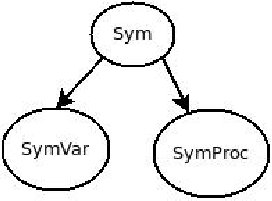
\includegraphics[scale=0.5]{sym.jpg}}
    \caption{Sym}
    \label{fig sym}
  \end{figure}
  
  \begin{itemize}
  \item \textbf{SymVar:}      
    Representa un s\'imbolo de una variable de algun tipo, tanto b\'asico, como compuesto. El atributo \emph{isConst} indica si el identificador fue declarado como variable o 
    constante. En cambio el atributo \emph{offset} determina cual es el desplazamiento de la variable con respecto al marco de pila(Frame Pointer) o al bloque de memoria est\'atico, dependiendo \'esto de si la variable es global o no.
    
  \item \textbf{SymProc:}      
    Representa un s\'imbolo de una subrutina, tanto procedimiento como funci\'on. Sus atributos son una lista llamada \emph{in} que guarda los parametros de entrada de la subrutina, \emph{ref} que es una lista que contiene booleanos indicando si los argumentos son por referencia o no,
    \emph{tamlocal} que es el tamaño en bytes que se necesita para las variable locales y un bloque de instrucciones con el cuerpo de la subrutina. El atributo \emph{bloque} es el que contiene la tabla de s\'imbolos del procedimiento con las declaraciones locales al mismo.
  \end{itemize}
\item \textbf{AST:}
  Los \'arboles sint\'acticos se implementaron por medio de varias clases con la siguiente jerarqu\'ia:\\
  
  \begin{figure}[htp]
    \centering
    \mbox{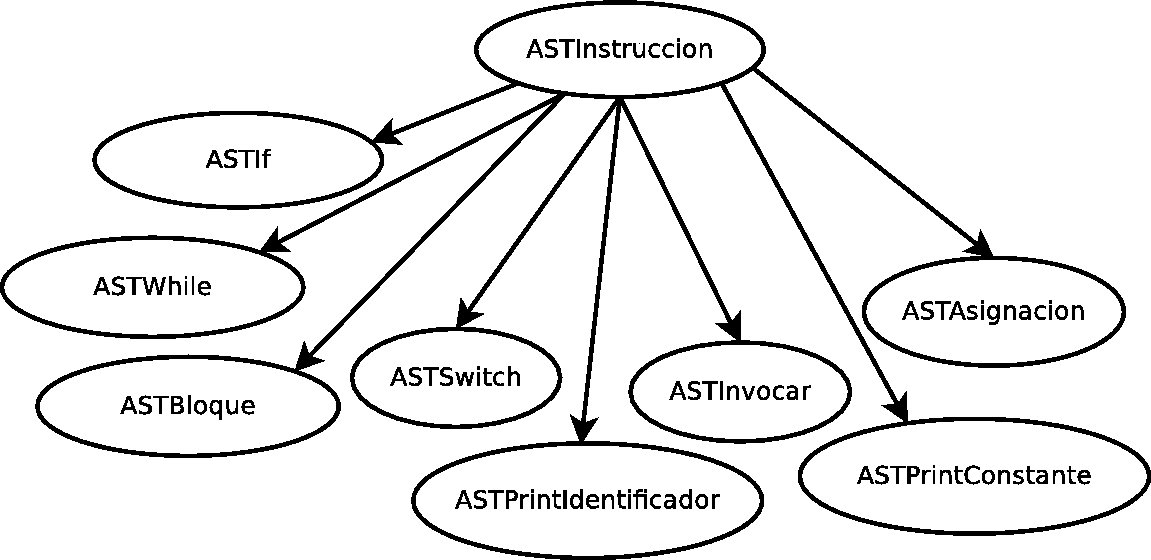
\includegraphics[scale=0.5]{instrucciones.jpg}}
    \caption{Arbol de herencia de las instrucciones}
    \label{fig instrucciones}
  \end{figure}
  
  La clase padre ASTInstrucci\'on, tiene tres atributos. Dos booleanos que indican si retorna o hace break. El \'ultimo atributo es un String con el nombre de la instrucci\'on. 
  
  El m\'etodo \emph{update} se encarga de verificar si la instrucci\'on retorna o hace break dentro de su cuerpo, y de actualizar los atributos de la clase que manejan estos casos.\\

  La mayor\'ia de las clases poseen un atributo Tipo llamado state que permite saber si hay errores, de que tipo son las expresiones, si las instrucciones estan bien. 
  Como su nombre lo dice lleva el estado de los \'arboles.\\
  
  \begin{itemize}
  \item \textbf{ASTAsignacion:}
    Consta de tres campos:
    \begin{itemize}      
    \item LinkedList ids: lista de ASTIdentificadores.
    \item LinkedList casts: lista de ASTCast.
    \item ASTExpresion expr: expresi\'on que se va a asignar.
    \item boolean isDeclaration: indica si la asignacion es de una declaraci\'o.
    \end{itemize}
  \item \textbf{ASTInvocar:}
    Consta de cuatro campos:
    \begin{itemize}      
    \item String nombre: nombre de la subrutina que se quiere llamar.
    \item LinkedList expresionEntrada: lista de ASTExpresion, con los argumentos de entrada.
    \item Tipo state: tipo del valor que devuelve la subrutina.
    \end{itemize}

    El m\'etodo \emph{check} de esta clase, s\'olo es llamado cuando ya se sabe que la subrutina que se quiere invocar ha sido declarada anteriormente.
  \item \textbf{ASTIf:}
    Consta de tres campos:
    \begin{itemize}
    \item LinkedList cond: cada uno de las expresiones booleanas que se tienen en los if y elif.
    \item LinkedList bloques: los bloques de c\'odigo de los if y elif.
    \item ASTBloque els: El bloque de c\'odigo del else.
    \end{itemize}
  \item \textbf{ASTWhile:}
    Sus campos son:
    \begin{itemize}
    \item ASTExpresion cond: condici\'on que debe cumplir para estar en el ciclo.
    \item ASTBloque bloque: bloque de c\'odigo a ejecutar.
    \end{itemize}
  \item \textbf{ASTBloque:}
    \begin{itemize}
    \item SymTable table: Tabla de s\'imbolos correspondiente del bloque.
    \item LinkedList insts: Lista de las instrucciones.
    \end{itemize}
  \item \textbf{ASTIdentificador:}
    \begin{itemize}
    \item SymTable table: Tabla donde se encontr\'o el identificador.
    \item ASTAcceso acceso: El acceso que se le haga al identificador ([] de arreglo o . de campo de un registro o uni\'on).
    \end{itemize}
  \item \textbf{ASTSwitch:}
    Sus atributos son:
    \begin{itemize}
    \item ASTExpresion exp: La expresi\'on del switch.
    \item LinkedList cases: Lista de ASTConst, con cada una de las constantes de los cases.
    \item LinkedList bloques: Lista de ASTBloque, con cada uno de los bloques de los cases.
    \item ASTBloque def: ASTBloque del caso default.
    \end{itemize}
  \item \textbf{ASTReturn:}
    Sus atributos son:
    \begin{itemize}
    \item int offset: Desplazamiento con respecto al FP, donde se tiene que colocar el valor de retorno.
    \end{itemize}


    Para ver que est\'an bien lo que se revisa es que cada uno de los bloques este bien. Adem\'as se ve que el tipo de la expresi\'on corresponda con cada una de las constantes.

  \item \textbf{ASTExpresi\'on:}    
    Posee los siguientes atributos:
    \begin{itemize}
    \item String value: Nombre del operador principal de la expresi\'on.
    \item Tipo state: tipo de la expresi\'on.
    \item ASTExpresion left: Expresi\'on izquierda.
    \item ASTExpresion right: Expresi\'on derecha.  En el caso que sea unitaria \'esta es nula.
    \end{itemize}

    Esta clase tiene el m\'etodo \emph{update} que se encarga de actualizar el campo \emph{state} de la expresi\'on y el m\'etodo \emph{check} que indica si dicha expresi\'on
    es v\'ailida o no.

    \begin{figure}[htp]
      \centering
      \mbox{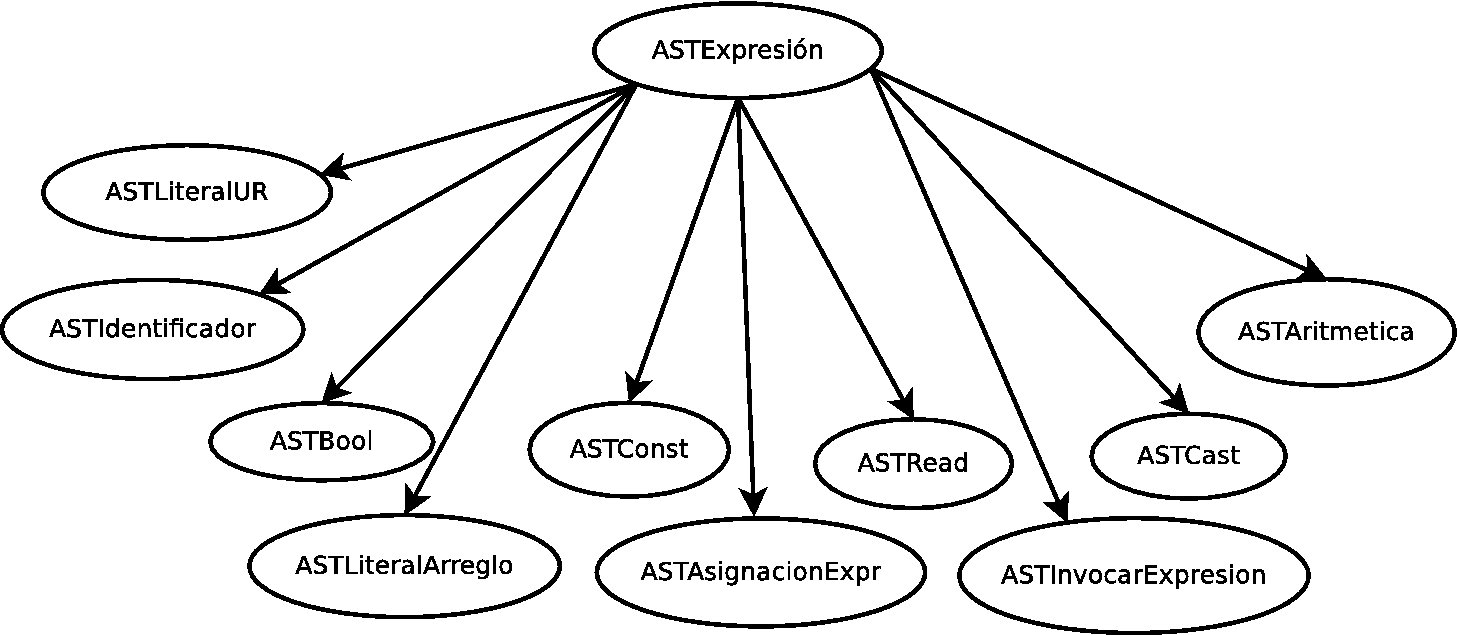
\includegraphics[scale=0.4]{expresiones.jpg}}
      \caption{Herencia de la clase ASTExpresion}
      \label{fig expresion}
    \end{figure}
    
  \item \textbf{ASTAsignacionExpr:}
    \begin{itemize}
    \item ASTIdentificador id: Identificador al que se asigna la expresi\'on en cuesti\'on.
    \item ASTCast cast: Indica si hay que hacerle una conversi\'on al tipo de la expresi\'on.
    \end{itemize}

    Esta clase s\'olo es usada para adornar los \'arboles de expresiones, por lo que en el caso de una asignaci\'on o a la hora de empilar parametros los casts se tienen que generar. El problema por el cual no se adorn\'o todo es porque existe la asignaci\'on m\'ultiple y la de tipos compuestos, donde los casteos son mucho m\'as complicados.

  \item \textbf{ASTInvocarExpresi\'on:}
    Contiene los mismo tres campos que ASTInvocar.
  \item \textbf{ASTAritm\'etica:}    
    Tiene dos \'arboles, de los cuales uno puede ser nulo en el caso que la operaci\'on sea unaria.
  \item \textbf{ASTBool:}    
    Es igual a la clase ASTArim\'etica, s\'olo que difiere en los chequeos que realiza: las expresiones que se pueden comparar son diferentes a 
    las que se pueden sumar, restar, dividir, etc.
  \item \textbf{ASTConst:}    
    Se usa para almacenar las constantes, por cuatro campos: entero, flotante, caracter y booleano. Cuando se crea se le asigna un valor a uno de estos.

  \item \textbf{ASTAcceso:}    
    Esta clase representa los posibles accesos que se le pueden hacer a un identificador ([] o .).\\

    El \'unico atributo de la clase denotado por el identificador \emph{hijo}, se utiliza para manejar n cantidad de accesos seguidos a un mismo identificador.

    Sus subclases son las siguientes:

    \begin{figure}[htp]
      \centering
      \mbox{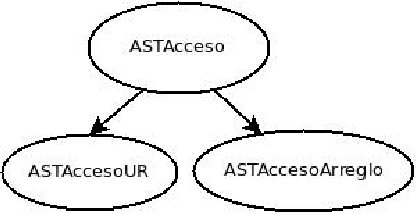
\includegraphics[scale=0.5]{acceso.jpg}}
      \caption{Herencia de la clase ASTAcceso}
      \label{fig acceso}
    \end{figure}

  \item \textbf{ASTAccesoUR:}    
    Representa el acceso a un campo de un registro o una uni\'on. Por ello s\'olo tiene un String que contiene el campo que se quiere accesar.    
  \item \textbf{ASTAccesoArreglo:}
    Como su nombre lo dice representa el acceso a un arreglo. Su \'unico atributo es una ASTExpresion que representa el \'indice del arreglo que se quiere acceder.
  \item \textbf{ASTPrintConstante:}
    Sus atributos son:
    \begin{itemize}
    \item ASTConst constante: La constante que se quiere imprimir.
    \end{itemize}

  \item \textbf{ASTPrintIdentificador:}
    Sus atributos son:
    \begin{itemize}
    \item ASTIdentificador iden: El identificador que se quiere imprimir.
    \end{itemize}

  \item \textbf{ASTRead:}
    \'Esta clase no tiene atributos, y se crean instancias de la misma para que a la hora de generar c\'odigo de dicha instrucci\'on, se sepa que \'esta es una
    instrucci\'on de lectura.\\

  \item \textbf{ASTCast:}
    Es una clase para ``adornar'' los AST de algunas expresiones básicas. Se crean instancias de \'esta clase para saber cuando debe hacerse la traducci\'on 
    necesaria para la transformaci\'on de un tipo de dato b\'asico a otro b\'asico tambi\'en.

  \item \textbf{ASTLiteralArreglo:}
    Sus atributos son:
    \begin{itemize}
    \item LinkedList arreglos: lista de listas que contiene el literal que se quiere asignar.
    \item boolean flag: indica si ha ocurrido un error revisando el literal.
    \end{itemize}

  \item \textbf{ASTLiteralUR:}
    Sus atributos son:
    \begin{itemize}
    \item LinkedList asignaciones: son las asignaciones que se le quieren hacer a una estructura o uni\'on.
    \end{itemize}
  \end{itemize}
\end{itemize}

\textbf{Funcionamiento general:}\\

La idea es ir verificando todo lo que se puede a medida que se va parseando. Por eso se tienen en los \'arboles los m\'etodos update y check. El primero lo que va 
a hacer es ver como quedaron los \'arboles abajo de \'el y a partir de ello en la variable state se indica si se encontr\'o un error (en ese caso state es null) o sino 
en que estado qued\'o.\\ 

\textbf{Ejemplo 1:}\\

De la expresi\'on 

\begin{verbatim}
true == (a+b > 1*1.25) 
\end{verbatim}

resulta el siguiente \'arbol:

\begin{figure}[htp]
  \centering
  \mbox{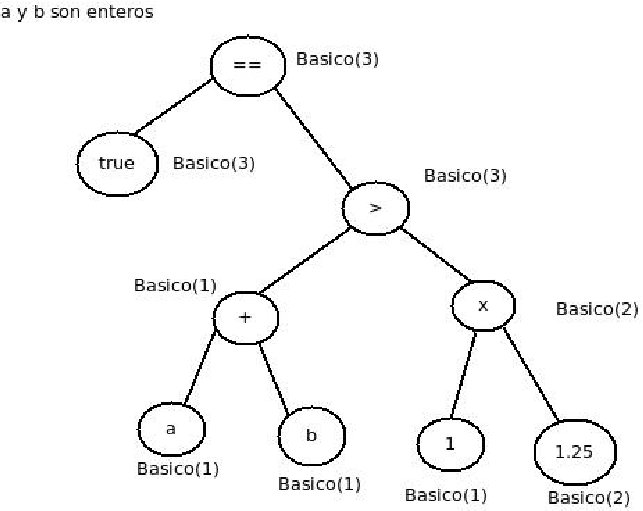
\includegraphics[scale=0.5]{arbol.jpg}}
  \caption{Ejemplo de construcci\'on y chequeo de \'arboles}
  \label{fig arbol}
\end{figure}

Todo esto se va haciendo a medida que se ejecutan las reglas en la gram\'atica.\\

En cuanto a las delcaraciones, \'estas van a ser almcenadas en las tablas de s\'imbolos y adem\'as son traducidas como asignaciones para construir su \'arbol correspondiente.\\

Otro detalle es que para lograr tener las declaraciones anidadas, lo que se hizo es tener dos tablas de s\'imbolos: la actual y la anterior. Entonces siempre 
que se entre a un bloque, la tabla actual se vuelve una nueva, y la anterior la actual. Al salir vuelven al estado original.\\

\textbf{Ejemplo 2:}\\

Se tiene:

     \begin{verbatim}
	struct {
	  float campo1;
	}[5] a;

	a[1].campo1 == 5
     \end{verbatim}

\newpage 
El \'arbol que se construye de la expresi\'on dada es el siguiente:\\

\begin{figure}[htp]
  \centering
  \mbox{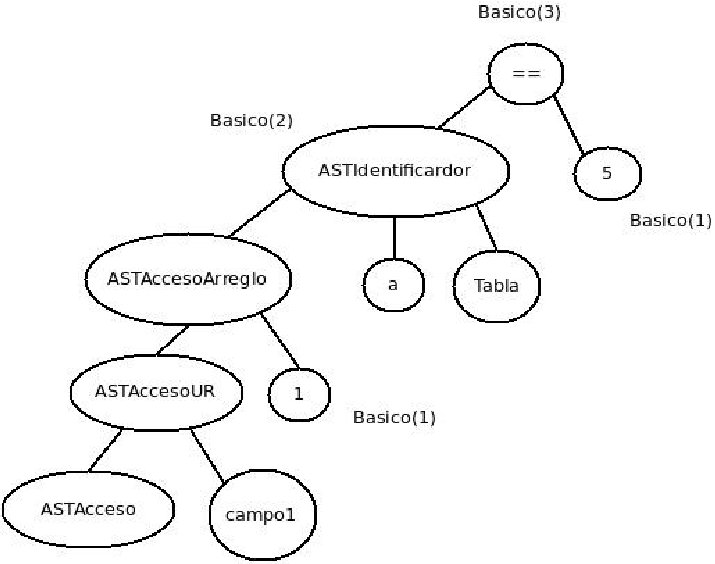
\includegraphics[scale=0.5]{arbol2.jpg}}
  \caption{Ejemplo de construcci\'on y chequeo de \'arboles}
  \label{fig arbol2}
\end{figure}

En los accesos se calcula el tipo resultante, en este caso un flotante. Luego se revisa si es posible equivaler eso con un entero, cosa que es posible.\\

Para calcular el tipo resultante de un acceso lo que se hace es ver el \'arbol de Tipo de \emph{a}:

\begin{figure}[htp]
  \centering
  \mbox{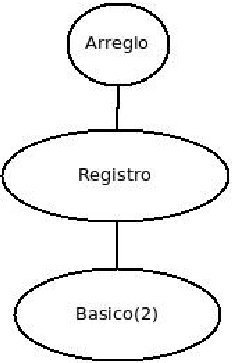
\includegraphics[scale=0.5]{arbolTipo.jpg}}
  \caption{Arbol de tipo de la variable a}
  \label{fig arbolTipo}
\end{figure}

Se recorre al mismo tiempo que el \'arbol de acceso, con lo que se puede determinar si el acceso es v\'alido y cual es su resultado.

\subsection{Generaci\'on de c\'odigo}
Se decidi\'o que el c\'odigo a generar es para arquitecturas de 64-bits, para ello se usan las instrucciones y sint\'axis adecuada siguiendo la documentaci\'on de NASM.\\

Los registros del lenguaje son los siguientes: \emph{rax, rbx, rcx, rdx, rdi, rsi, r8, r9, r10, r11, r12, r13, r14 y r15}. El stack pointer y el frame pointer son 
\emph{rsp y rbp} respectivamente.\\

Esta informaci\'on se tiene en una clase est\'atica llamada \emph{AssemblerInfo}. Adem\'as \'esta pos\'ee procedimientos para salvar y restaurar registros, generar 
el c\'odigo inicial del archivo de salida, entre otras.\\

Por otro lado cada uno de los AST tiene un m\'etodo llamado \emph{generateCode}; dependiendo de la clase, el n\'umero y tipo de par\'ametros var\'ia. En el caso de 
las instrucciones, dicho m\'etodo posee cuatro par\'ametros: el primero es el descriptor del archivo de salida donde se va a escribir el c\'odigo ensamblador, el segundo 
es el n\'umero de registro disponible para usar dentro de la generaci\'on de c\'odigo de dicha instrucci\'on, el tercero el nombre de la etiqueta cuando se quiere hacer un break y el \'ultimo la etiqueta a donde hacer el salto de retorno de una funci\'on o procedimiento. \\

Para obtener nuevas etiquetas se hace uso de \emph{newLabel} en la clase AssemblerInfo.

En el caso del ASTif el código de genera de la siguiente forma:

\begin{verbatim}

  Iterator itc = cond.iterator();
  Iterator itb = bloques.iterator();

  String si = AssemblerInfo.newLabel();
  String no = AssemblerInfo.newLabel();
  String end = AssemblerInfo.newLabel();

  ((ASTExpresion) itc.next()).generateCode(fd,nextReg, si, no);
  fd.write(si + ":\n");
  ((ASTBloque) itb.next()).generateCode(fd, nextReg);
  fd.write("jmp " + end + "\n");

  while(itc.hasNext()) {
    si = AssemblerInfo.newLabel();
    fd.write(no + ":\n");
    no = AssemblerInfo.newLabel();
    ((ASTExpresion) itc.next()).generateCode(fd, nextReg, si, no);
    fd.write(si + ":\n");
    ((ASTBloque) itb.next()).generateCode(fd, nextReg);
    fd.write("jmp " + end + "\n");
  }

  fd.write(no + ":\n");
  if(els != null)
    els.generateCode(fd, nextReg);

  fd.write(end + ":\n");

\end{verbatim}

\'Este funciona del siguiente modo: \\
  \begin{itemize}
  \item
  Se genera el c\'odigo del primer if ( este siempre va a estar ). Para ellos se llama al primer condicional del iterador. Se genera el c\'odigo del 
  primer condicional. Se ve que se le pasan las dos etiquetas de salto ya que es una expresi\'on booleana. Posterior se coloca la etiqueta si y el 
  c\'odigo a ejecutar del if, con un salto al final. \'Esto son las siguientes l\'ineas:

  \begin{verbatim}
    ((ASTExpresion) itc.next()).generateCode(fd,nextReg, si, no);
    fd.write(si + ":\n");
    ((ASTBloque) itb.next()).generateCode(fd, nextReg);
    fd.write("jmp " + end + "\n");
  \end{verbatim}

  \item
  Luego se tienen que generar el c\'odigo de las expresiones y bloques de los \emph{elif}. \'Esto es seguir recorriendo el iterador de los condicionales 
  y bloques. A medida que se hace \'esto se va generando el c\'odigo. Se sigue el mismo esquema que se uso para el primer condicional, s\'olo que hay
  que agregar la etiqueta no para cuando una expresi\'on booleana falle, salte a la siguiente. Corresponde a la siguiente parte:

  \begin{verbatim}
    while(itc.hasNext()) {
      si = AssemblerInfo.newLabel();
      fd.write(no + ":\n");
      no = AssemblerInfo.newLabel();
      ((ASTExpresion) itc.next()).generateCode(fd, nextReg, si, no);
      fd.write(si + ":\n");
      ((ASTBloque) itb.next()).generateCode(fd, nextReg);
      fd.write("jmp " + end + "\n");
    }
  \end{verbatim}

  \item
  Finalmente ya s\'olo queda generar el c\'odigo del else en el caso que se encuentre. Para ello se revisa que no sea nulo, y en el caso que se cumpla
  \'esto se genera su c\'odigo. Y se coloca la etiqueta end, que es para cuando se halla ejecutado un bloque salte al final de todo el if. 
  Ser\'ia lo siguiente:

  \begin{verbatim}
    fd.write(no + ":\n");
    if(els != null)
      els.generateCode(fd, nextReg);

    fd.write(end + ":\n");
  \end{verbatim}

  \end{itemize}

En el caso del switch, while y for es muy parecedio a \'esta generaci\'on de c\'odigo. En el caso del switch no hay ning\'un tipo de optimizaci\'on.
El while tiene una peque\~na optimizaci\'on pensando en el pipelining que tiene el procesador. Consiste en lo siguiente: primero \'esta el c\'odigo
del bloque, luego viene una etiqueta y finalmente la expresi\'on booleana. As\'i se disminuye el n\'umero de saltos necesarios.\\

La asignaci\'on si es mucho mas complicada ya que en el lenguaje se permite el uso de accesos y el poder asignar tipos complejos. Por lo que el c\'odigo
es super extenso y toma en cuanta muchos casos: asignar un identificador, un literal, una expresion booleana, los cast que hay que hacer, retorno de una funci\'on, entre otras cosas.\\

En el caso del break y return es simplemente generar una etiqueta que salte a los parametros que le llegan. El return si es mas complejo ya que requiere en el caso que se encuentre en una funci\'on el colocar en el espacio de la pila para el retorno el valor de \'esta. Por lo que el c\'odigo 
es el mimso de la asignaci\'on con un salto.\\

En el caso de la invocaci\'on de un procedimiento o funci\'on se siguen las siguientes convenciones:

  \begin{itemize}
  \item \textbf{Llamador}: A partir del par\'ametro que le indica que registro puede usar, salva los registros necesarios. Por ejemplo si el n\'umero
  del pr\'oximo registro es el 5, entonces salva los primero 5 registros. Luego se encarga de empilar los parametros. Llama a la func\'on. Desempila
  los par\'ametros. En el caso que tenga un valor de retorno, si este no es booleano simplemente lo deja en la pila. Y finalmente restaura los registros.
  \item \textbf{Llamado}: Primero guarda la direcci\'on de retorno en la pila, luego el FP y lo actualiza. Despu\'es aumenta la pila con respecto a las variables locales. En esta implementaci\'on no se salvan registros ya que no se hace uso de registros para variables locales. Al salir se quita de la pilas las variables locales, se restaura el antiguo FP y se salta a la direcci\'on de retorno.
  \end{itemize}

El m\'etodo de generaci\'on de c\'odigo de las expresiones tiene \'estos mismos dos par\'ametros descritos anteriormente, a los que se le suman otros dos, que son usados 
por las expresiones booleanas. Ambos representan ``etiquetas'', de \emph{si} y \emph{no}, que indican a que parte del c\'odigo se debe saltar, si la expresi\'on es verdadera,
o falsa.\\

En este caso el problema en que se incurri\'o fueron los flotantes. Tanto para las expresiones aritm\'eticas como para las booleanas se tuvo que 
generar un c\'odigo especial, donde se hace uso del FPU. Tambi\'en como las expresiones booleanes simpre hacen un salto en vez de retornar el valor
Esto agrego muchos casos. \\

La generaci\'on de c\'odigo para una expresi\'on aritm\'etica binaria es la siguiente:\\

  \begin{verbatim}
    String reg = AssemblerInfo.getNombresRegAtPos(nextReg);
    String nreg = AssemblerInfo.getNombresRegAtPos(nextReg+1);	

    left.generateCode(fd, nextReg, si, no);		    
	AssemblerInfo.saveReg(fd, nextReg + 1);
	right.generateCode(fd, nextReg + 1, si, no);
	fd.write(OPERACION + reg + ", " + nreg + "\n");		
    AssemblerInfo.restoreReg(fd, nextReg + 1);

  \end{verbatim}

Lo que se hace es simple: se genera el c\'odigo del lado izquierdo usando el registro que se le asign\'o. Luego se llama el m\'etodo saveReg de la 
clase AssemblerInfo, que revisa el n\'umero del registro que se est\'a usando y de ser este mayor al n\'umero total de registros genera c\'odigo para
salvarlo. Luego se genera la expresi\'on del lado derecho usando el siguiente registro, por eso el nextReg +1. Finalmente lo que queda es hacer la operaci\'on entre los registros. Cabe actora que el m\'etodo getNombresRegAtPos da el String del registro a partir de su n\'umero. Y bueno al final
de ser necesario se restaura el registro, es exactamente el opuesto al m\'etodo saverReg.\\

En el caso de los flotantes se tienen que cargar los valores a la pila de registros del FPU y hacer la operaci\'on adecuada y devolver el valor.\\

Se hace lo siguiente:\\

  \begin{verbatim}
    String reg = AssemblerInfo.getNombresRegAtPos(nextReg);
    String nreg = AssemblerInfo.getNombresRegAtPos(nextReg+1);	

	left.generateCode(fd, nextReg, si, no);		    
	AssemblerInfo.saveReg(fd, nextReg + 1);
	right.generateCode(fd, nextReg + 1, si, no);
			
	fd.write("push "+reg+"\n");
	fd.write("fld qword ["+AssemblerInfo.getSp()+"]\n");
		
	fd.write("push "+nreg+"\n");
	fd.write("OPERACION qword ["+AssemblerInfo.getSp()+"]\n");
			
	fd.write("fstp qword ["+AssemblerInfo.getSp()+" + 8]\n");
		    
	fd.write("pop " + nreg + "\n");
	fd.write("pop " + reg + "\n");
		    
	AssemblerInfo.restoreReg(fd, nextReg + 1);

  \end{verbatim}

Es parecido al caso de los enteros, pero en este caso se tienen que cargar los valores del FPU y s\'olo se puede hacer desde memoria. Al igual se
genera el c\'odigo del lado izquierdo. Se salva el registro si es necesario, se genera el lado derecho. Ahora hace push del registro con el primer
resultado. Se carga ese valor al FPU mediante la instrucci\'on fld. Luego se coloca en memoria el segundo operando y se hace la operaci\'on. Finalmente
se coloca el resultado en memoria, en este caso en la posici\'on de memoria donde se encuentra el primer registro empilado, con el objetivo que cuando 
se haga pop de el ya tenga el resultado en \'el.

En el caso de las expresiones booleanas,  \emph{generateCode} se van a ver tres casos cuando se compara enteros o caracteres, flotantes
y booleanos. Cada uno tiene su forma de generar el c\'odigo. En cuanto a las aritm\'eticas simplemente estan el caso de los flotantes y enteros.\\

Por \'ultimo como detalle importante es que cuando se usa una funci\'on como expresi\'on esta va a dejar empilado su valor de retorno, exceptuando en el caso que sea un booleano.\\

\subsection{C\'alculo de desplazamiento de variables}

Para las variables globales simplemente se calcula el espacio que van a usar ya que \'estas pueden ser usadas en cualquier parte del c\'odigo. Y \'este espacio es 
reservado est\'aticamente. En el archivo de salida, a este espacio se le asocia el identificador ``static''.\\

Por otro lado lo que se hace con las locales es calcular cual es la mayor cantidad de memoria que se va a necesitar en el programa siguiendo una cadena de bloques. 
Para ello se lleva en una variable ``desplazamiento'', el espacio de cada variable declarada; junto con \'esta variable, se usa una pila de enteros de la siguiente 
forma: cuando se entre un bloque nuevo se salva el valor del desplazamiento que se llevaba y al salir se recupera. De este modo se consume menos memoria y adem\'as 
se evita el problema de tener que estar empilando variables, que diferencia de las globales, se almacenan en la pila.\\

\textbf{Ejemplo :}\\

\begin{verbatim}
int a,b,c;
float d;

int main {
  int x,y,z;

  if (...) {
     int j,k,l;
     while (...) {
       int t,y,u;
     }
  }
  else {
     int o,p;
  }
}
\end{verbatim}

Para \'este caso se van a reservar 32 bytes para las variables globales, que corresponen a 8 bytes por cada una de las siguientes variables: a, b, c y d; y 72 bytes para el \emph{main}
y sus respectivas variables locales, que en el peor de los casos, si el flujo del programa se va por la rama del \emph{if}, se requerir\'a espacio para las siguientes variables: x, y, 
z, j, k, l, t, y, u.\\

\section{Casos de prueba}

\subsection{Criterios Generales}

\begin{itemize}
\item Los tipos de prueba que se van a hacer principalmenteson de caja negra, es decir, del comportamiento observable y externo del sistema.
\item Se quiere simular las situaciones m\'as comunes de un programador usando el lenguaje.
\item An\'alisis de los casos bordes.
\end{itemize}

A continuaci\'on se muestran todos los casos de pruebas con sus respectivas intenciones y salidas esperadas.\\

\begin{itemize}

\item \textbf{Break:}\\ \\
  \emph{Intenci\'on:}\\ \\
  Ver que la generaci\'on de break esta bien hecha.\\ \\
  \emph{Casos:}\\ 
  \begin{table}[!hbp]
    \begin{tabular}{c c c c}
      \hline            
      \hline            
      Caso de Prueba & Objetivo                       & Salida Esperada      & Resultado \\ [0.5ex]
      \hline                          
      b1.lang        & Comprobar el uso de break      & I mpresi\'on de 3    & Correcto  \\ [1ex] 
                     & en un ciclo simple             &                      &           \\ [1ex] 
      b2.lang        & Comprobar el uso de break en   & I mpresi\'on de 0,0, & Correcto  \\ [1ex] 
                     & varios while anidados          & 1,2,3,4,5, true y    &           \\ [1ex] 
                     &                                & true                 &           \\ [1ex] 
      \hline
    \end{tabular}    
  \end{table}


\item \textbf{Llamadas:}\\ \\
  \emph{Intenci\'on:}\\ \\
  Ver que la generaci\'on de funciones y procedimientos funcione adecuadamente.\\ \\
  \emph{Casos:}\\ 
  \begin{table}[!hbp]
    \begin{tabular}{c c c c}
      \hline            
      \hline            
      Caso de Prueba & Objetivo                       & Salida Esperada      & Resultado \\ [0.5ex]
      \hline                          
      l1.lang        & Se quiere ver que las llamadas & I mpresi\'on de a,3, & Correcto  \\ [1ex] 
                     & a funciones simples est\'an    & a,7 y 9              &           \\ [1ex] 
                     & funcionando                    &                      &           \\ [1ex] 
      l2.lang        & Comprobar que efictavamente    & I mpresi\'on de 3,5, & Correcto  \\ [1ex] 
                     & los par\'ametros son pasados   & a y 3                &           \\ [1ex] 
                     & por valor y que pueden ser     &                      &           \\ [1ex] 
                     & modificados dentro del proce-  &                      &           \\ [1ex] 
                     & dimiento                       &                      &           \\ [1ex] 
      l3.lang        & Comprobar el pasaje por        & I mpresi\'on de 3,3, & Correcto  \\ [1ex] 
                     & valor/resultado                & 2 y 2                &           \\ [1ex] 
      l4.lang        & Ver que se hacen los casts en  & I mpresi\'on de 3.0  & Correcto  \\ [1ex] 
                     & la llamada                     &                      &           \\ [1ex] 
      l5.lang        & Ver que los casts esten        & I mpresi\'on de 3.0, & Correcto  \\ [1ex] 
                     & con los parametros valor/re-   & 4.2 y 4              &           \\ [1ex] 
                     & sultado                        &                      &           \\ [1ex] 
      \hline
    \end{tabular}    
  \end{table}

  \newpage

  \begin{table}[!hbp]
    \begin{tabular}{c c c c}
      \hline            
      \hline            
      Caso de Prueba & Objetivo                       & Salida Esperada      & Resultado \\ [0.5ex]
      \hline                          
      l6.lang        & Pasaje de parametros de un     & I mpresi\'on de 1    & Correcto  \\ [1ex] 
                     & arreglo sirve. Al igual que    &                      &           \\ [1ex] 
                     & el uso de literales.           &                      &           \\ [1ex] 
      l7.lang        & El pasaje de parametros de     & I mpresi\'on de 3    & Correcto  \\ [1ex] 
                     & literales es el adecuado       &                      &           \\ [1ex] 
      l8.lang        & Comprobar el pasaje por va-    & I mpresi\'on de 5    & Correcto  \\ [1ex] 
                     & lor/resultado de estructuras   &                      &           \\ [1ex] 
                     & complejas                      &                      &           \\ [1ex] 
      l9.lang        & Comprobar que la recursión y   & I mpresi\'on del     & Correcto  \\ [1ex] 
                     & el return con tipos básicos    & factorial n\'umero   &           \\ [1ex] 
                     & sirve                          & dado                 &           \\ [1ex] 
      l10.lang       & Comprobar que la recursión y   & I mpresi\'on del     & Correcto  \\ [1ex] 
                     & el return con tipos básicos    & fibonacci n\'umero   &           \\ [1ex] 
                     & sirve                          & dado                 &           \\ [1ex] 
      l11.lang       & el return de tipos comlejos    & I mpresi\'on  4, 11, & Incorrecto: Falla en la  \\ [1ex] 
                     & sirve                          & 2.03 y h.            & generaci\'on de c\'odigo  \\ [1ex] 
      \hline
    \end{tabular}    
  \end{table}

\item \textbf{Complejos:}\\ \\
  \emph{Intenci\'on:}\\ \\
  Ver que los accesos y asignaciones a los complejos funcionan de forma correcta\\

  \emph{Casos:}\\ 

  \newpage
  \begin{table}[!hbp]
    \begin{tabular}{c c c c}
      \hline            
      \hline            
      Caso de Prueba & Objetivo                        & Salida Esperada      & Resultado \\ [0.5ex]
      \hline                          
      c1.lang        & Se desea comprobar que la       & I mpresi\'on de true & Correcto  \\ [1ex] 
                     & instrucci\'on hasctive funcione &                      &           \\ [1ex] 
      c2.lang        & Se quiere comprobar que las     & I mpresi\'on de 2,3, & Correcto  \\ [1ex] 
                     & asignaciones en los arreglos    & 4 y 1                &           \\ [1ex] 
      c3.lang        & Ver que se indican los errores  & I mpresi\'on del     & Correcto  \\ [1ex] 
                     & de indexaci\'on                 & error                &           \\ [1ex] 
      c4.lang        & Las asignaciones en los arre-   & I mpresi\'on de 3 y  & Correcto  \\ [1ex] 
                     & glos funcionan y además que se  & 8 seguido de un      &           \\ [1ex] 
                     & indique si se sale del \'indice & error                &           \\ [1ex] 
      c5.lang        & Comprobar que las asignaciones  & I mpresi\'on de 16,  & Correcto  \\ [1ex] 
                     & en estrucutras, arreglos y u-   & true y 0.02          &           \\ [1ex] 
                     & niones funcionan adecuadamente. &                      &           \\ [1ex] 
                     & Además del uso de literales     &                      &           \\ [1ex] 
      c6.lang        & Ver que se indican en los e-    & I mpresi\'on de      & Correcto  \\ [1ex] 
                     & rrores a la hora de usar un     & error                &           \\ [1ex] 
                     & campo de la uni\'on que no      &                      &           \\ [1ex] 
                     & est\'a activo.                  &                      &           \\ [1ex] 
      \hline
    \end{tabular}    
  \end{table}

\item \textbf{Oficiales:}\\ \\
  \emph{Intenci\'on:}\\ \\
  Estos son los casos de prueba obligarios para tods los grupos traducidos a este lenguaje espec\'ifico.\\

  \emph{Casos:}\\
  \newpage

  \begin{table}[!hbp]
    \begin{tabular}{c c c c}
      \hline            
      \hline            
      Caso de Prueba              & Objetivo               & Salida Esperada & Resultado \\ [0.5ex]
      \hline                          
      fibIterativo.lang           & Calcular de forma ite- & N\'umero de fibonacci & Correcto                    \\ [1ex] 
                                  & rativa el n\'umero de  & de n\'umero ingresado &                             \\ [1ex] 
                                  & fibonacci de cierto    & por c\'onsola por el  &                             \\ [1ex] 
                                  & n\'umero que se pide   & usuario.              &                             \\ [1ex] 
                                  & por c\'onsola al usu-  &                       &                             \\ [1ex]   
                                  & ario.                  &                       &                             \\ [1ex]   
      fibLogaritmico.lang         & Calcular de forma lo-  & N\'umero de fibonacci & Correcto                    \\ [1ex] 
                                  & gar\'itmica el n\'umero& de n\'umero ingresado &                             \\ [1ex] 
                                  & de fibonacci de cierto & por c\'onsola por el  &                             \\ [1ex] 
                                  & n\'umero que se pide   & usuario.              &                             \\ [1ex] 
                                  & por c\'onsola al usu-  &                       &                             \\ [1ex]   
                                  & ario.                  &                       &                             \\ [1ex]   
      generarPermutaciones.lang   & Generar todas las posi-& Se imprime por c\'on- & Correcto                    \\ [1ex] 
                                  & bles permutaciones de  & sola todas las posi-  &                             \\ [1ex] 
                                  & un arreglo de caracte- & bles permutaciones del&                             \\ [1ex] 
                                  & res que se pide por    & arreglo ingresado.    &                             \\ [1ex] 
                                  & c\'onsola.             &                       &                             \\ [1ex] 
      multiplicacionMatrices.lang & Calcular la multiplica-& Se imprime por c\'on- & Correcto                    \\ [1ex]
                                  & ci\'on de una matriz de& sola el resultado de  &                             \\ [1ex] 
                                  & flotantes y una matriz & la multiplicaci\'on de&                             \\ [1ex] 
                                  & de enteros almacenadas & una matriz de flotan- &                             \\ [1ex] 
                                  & en una estructura.     & tes y una matriz de en&                             \\ [1ex] 
                                  &                        & teros.                &                             \\ [1ex] 
      raizCuadrada.lang           & Calcular la ra\'iz cua-& Se imprime por c\'on- & El programa se ejecuta sin  \\ [1ex] 
                                  & drada de un flotante   & sola la ra\'iz cuadra-& problemas, pero los valores \\ [1ex]
                                  & que se pide por c\'on- & da del flotante pedido& aproximados de la ra\'iz cu-\\ [1ex] 
                                  & sola.                  &                       & adrada no son buenos.       \\ [1ex]  
      saludFinanciera.lang        &                        &                       & El programa se ejecut\'o    \\ [1ex]  
                                  &                        &                       & sin problemas, es posible   \\ [1ex] 
                                  &                        &                       & es posible que tenga errores\\ [1ex] 
                                  &                        &                       & la ejecuci\'on en vista que \\ [1ex] 
                                  &                        &                       & que siempre dio que la em-  \\ [1ex] 
                                  &                        &                       & presa es saludable.         \\ [1ex] 
      variantes.lang              &                        &                       & Correcto                    \\ [1ex] 
      \hline
    \end{tabular}    
  \end{table}

\end{itemize}

Para el caso de prueba de llamadas l5.lang se va ir mostrando paso a pasa la correctitud de \'este.\\

En el procedimiento principal que empieza con la etiqueta main primero se reserva memoria. Se reservan 8 
bytes dem\'as porque los desplazamientos empiezan en 8. El motivo es que no se puede tocar la secci\'on 
de memoria con desplazamiento 0, la cual ser\'ial [rbp], el motivo es que posiblemente se guarde algo
en esa regi\'on de memoria que es usado por las instrucciones enter y leave.\\

\begin{verbatim}
enter 16, 0
\end{verbatim}

Luego se le asigna el valor tres a la variable a. Para ellos se coloca el 3 en el registro rax y la direcci\'on
de memoria de a, que es 8 de desplazamiento con respecto al rbp y se le asigna el valor.\\

\begin{verbatim}
mov rax, 3
mov rbx, rbp
sub rbx, 8
mov [rbx], rax
\end{verbatim}

Posterior a \'esto viene el empilamiento de parametros para ello se hace lo siguiente. Primero como
se va a empilar la variable a, se saca su valor de la direcci\'on de memoria. Eso son las tres
primeras l\'ineas. Luego se transforma ese valor a un flotante, ya que ese es el tipo del par\'ametro de entrada, haciendo uso de las instrucci\'on
fild. Luego se empila ese valor, y como el parametro es por valor resultado se empila la direcci\'on de memoria y se llama al procedimiento.\\

\begin{verbatim}
mov rax, rbp
sub rax, 8
mov rbx, [rax]
push rbx
fild qword [rsp]
fstp qword [rsp]
pop rbx
push rbx
push rax
call procproc
\end{verbatim}

Despu\'es de la llamada se desempila la direcci\'on del registro en rax. Se saca el parametro en rbx y se procede a transformarlo a un entero.
Para ello se hace uso de la instrucci\'on fistp. Finalmente se almacena ese valor en la direcci\'on de memoria.\\

\begin{verbatim}
pop rax
pop rbx
push rbx
fld qword [rsp]
fistp qword [rsp]
pop rbx
mov [rax], rbx
\end{verbatim}

Queda por imprimir los valores para ello se salva el registro rdi, el cual es usado para pasar los parametros a imprimir a las funciones
correspondientes. Primero se coloca el valor de a y luego el n\'umero 10 que corresponde al salto de l\'inea en la tabla ascii.

\begin{verbatim}
push rdi
mov rax, rbp
sub rax, 8
mov rdi, [rax]
call print_int
pop rdi
push rdi
mov rdi, 10
call print_char
pop rdi
\end{verbatim}

En cuanto al c\'odigo del procedimiento que se llama, primero se reserva el espacio de memeria. En \'este caso no hay variables locales, pero
a pesar de eso se reservan 8 por lo dicho anteriormente de que los desplazamientos siempre van a comenzar en 8 por el problema que se tuvo.
Luego se procede a imprimir su valor por lo cual su direccion se encuentra 24 bytes por encima del rbp. Se llama a la funci\'on de imprimir.

\begin{verbatim}
enter 8, 0
push rdi
mov rax, rbp
sub rax, -24
mov rdi, [rax]
call print_float
pop rdi
push rdi
mov rdi, 10
call print_char
pop rdi
\end{verbatim}

Finalmente se le asigna el valir 4.2 a la variable a y se manda a imprimir. El valor 4.2 es transformado a un flotante de doble presici\'on el 
cual tiene como valor hexadecimal 0x4010cccccccccccd. Al terminar se ejecuta la instrucci\'on leave que es la opuesta a enter y la instrucci\'on
ret que desempila la direcci\'on de retorno y vuelve a donde antes estaba ejecutando.

\begin{verbatim}
mov rax, 0x4010cccccccccccd
mov rbx, rbp
sub rbx, -24
mov [rbx], rax
push rdi
mov rax, rbp
sub rax, -24
mov rdi, [rax]
call print_float
pop rdi
push rdi
mov rdi, 10
call print_char
pop rdi
label0:
leave
ret
\end{verbatim}

\newpage

\section{Problemas encontrados y soluciones propuestas}

El primer problema importante al que tuvimos que enfrentarnos fue que el uso de Java 1.4.2 complica el uso de tipos. Para se tuvo que hacer uso de muchos casts. \\

Tambi\'en el poco conocimiento de Jflex y JavaCup complic\'o en cierto modo el trabajo, ya que se perdi\'o una gran cantidad de tiempo aprendiendo a usar estas 
herramientas. En especial JavaCup que dio muchos errores de tipo a las hora de ir armando los \'arboles. Para ello se le tuvo que indicar a \'este, en la declaraci\'on
de los no terminales de la gram\'atica, qu\'e devolv\'ia cada producci\'on y \'el se encarga de hacer los casts.\\

Un problema que tuvimos que enfrentar en relaci\'on a la generaci\'on de c\'digo en general, fue que el manejo de la pila del lenguaje ensamblador s\'olo pudimos hacerlo
a trav\'es de las instrucciones de \emph{push} y \emph{pop}. Por alguna raz\'on que todav\'ia desconocemos, no pudimos modificar el \emph{stack pointer (rbp en NASM)} 
expl\'icitamente a trav\'es de instrucciones como \emph{add} o \emph{sub}.

\chapter{Detalles de compilaci\'on y corrida del lenguaje}
El uso es bastante simple una vez descargado el archivo, abra el terminal y vaya a la ubicaci\'on donde lo descarg\'o. Una vez hecho esto, va a necesitar 
descomprimir el archivo que esta en el formato .tar.gz. Para ello ejecute el siguente comando:\\

\begin{verbatim}
$> tar zxf nombre_archivo
\end{verbatim}

Luego se tiene que ejecutar un script de bash que se encargara de compilar todos los archivos y generar el archivo
de salida y adem\'as sejecutarlo.\\

\begin{verbatim}
$> sh makefile nombre_archivo_prueba nombre_archivo_salida
\end{verbatim}

Es importante destacar que debe darse toda la ruta del archivo de prueba que desee ejecutarse. Adem\'as, el archivo
de salida se creara con el nombre especificado por la c\'onsola, y se encontrar\'a dentro de la carpeta NAMS.\\

\chapter{Estado actual}
\section{Estado final del lenguaje}
En lineas generales nuestro lenguaje est\'a completamente operativo.\\

La gram\'atica ya est\'a completa y dise\~nada para los requisitos del trimestre pasado y esta segunda entrega. Se crean los \'arboles correspodientes para los tipos tanto b\'asicos
como compuestos y para las expresiones e instrucciones.\\

El lenguaje hace chequeos de variables no declaradas en su totalidad, siguiendo lo anteriormente mencionado en el caso de las instrucciones \emph{if},
\emph{for}, \emph{while} y \emph{switch}, donde las variables declaradas dentro de los bloques de cada una de estas instrucciones, s\'olo tendr\'an 
alcance dentro de \'estos mismos.\\

En cuanto al chequeo de tipos, se realizan chequeos de posibles coerciones v\'alidas entre tipos iguales y distintos para el caso de tipos b\'asicos, y las posibles
asignaciones para tipos compuestos, incluyendo asignaciones de literales para cada uno de los tipos compuestos.\\

En cuanto a la generaci\'on de c\'odigo, se logr\'o cubrir completamente la generaci\'on de c\'odigo de expresiones de todos los tipos b\'asicos y compuestos; incluyendo sus 
respectivos literales, as\'i como de las siguientes instrucciones: asignaci\'on, ambos condicionales \emph{If}, y \emph{Switch}, ambas iteraciones \emph{For} y \emph{While}, 
las instrucciones de E/S \emph{Print} y \emph{Read}, accesos a identificadores de tipo arreglo y compuestos y llamadas a procedimientos y funciones.\\

Tambi\'en cubrimos la declaraci\'on y llamada de funciones y procedimientos. Esto es, permitimos al programador hacer promesas de declaraci\'on
de subrutinas sin el cuerpo de las mismas, para permitir su uso y llamada dentro de otras subrutinas declaradas por debajo de ellas. Como consecuencia de \'esta
ventaja, se hace el chequeo correspondiente de la definici\'on del cuerpo de promesas de subrutinas hechas.\\

Actualmente no se maneja la E/S a trav\'es de archivos.\\

En la carpeta principal con los archivos del lenguaje, se encuentran tambi\'en varios casos de prueba que se utilizaron para probar los chequeos antes mencionados; as\' 
como los casos de prueba oficiales publicados. En lineas generales se hicieron casos de prueba donde se demuestra que los errores se estan detectando y mostrando por 
pantalla. Tambi\'en incluimos casos de prueba libres de errores.\\

\section{Errores}

Actualmente el uso de la instrucci\'on \emph{read char} dentro de alguna iteraci\'on para la iniciualizaci\'on de una variable de tipo \emph{Arreglo} de \emph{char}, no est\'a
funcionando correctamente. Lo que ocurre es que al pedir un caracter para la posici\'on \emph{i} por ejemplo, se guarda dicho caracter, pero al darle ``enter'', para
pedir el siguiente caracter para la posici\'on \emph{i+1}, se guarda el caracter \emph{``\n''} en esta \'ultima posici\'on.\\

Tambi\'en cabe destacar que el uso de expresiones booleanas que consten \'unicamente de un identificador, valga la redundancia, de tipo \emph{bool}, dentro de 
las condiciones de instrucciones como \emph{If}, \emph{Switch}, \emph{For} o \emph{While}, no funciona bien. As\'i como el pasaje de par\'ametros de tipo \emph{bool}, 
que cumpla con las mismas condiciones, es decir, \'unicamente un identificador.

\chapter{Conclusiones y recomendaciones}
Al ir dise\~nando e implementando cada uno de los detalles del lenguaje uno se va percatando lo complicado que es esta tarea. El hecho de tener que 
tomar en cuenta una gigantesca cantidad de aspectos para tratar de cumplir con la mayor cantidad posible de ellos, conlleva a veces ha  tomar decisiones err\'oneas. 
Uno se  puede desviar del objetivo principal del lenguaje. Por ello se recomienda no crear algo con una gran cantidad de opciones de tipos, instrucciones, etc., ya 
que esto por el contrario, puede traer como consecuencia un mal dise\~no del lenguaje, debido al gran tama\~no de la informaci\'on que debe manejarse.\\

Otro detalle que es importante mencionar es que una vez pasado a la fase de implementaci\'on del lenguaje, es bueno tener un dise\~no claro, para no estar constamente 
cambiando el c\'odigo. \'Esto puede reducir significativamente la cantidad de errores. Es preferible perder varias horas para tener un dise\~no lo mejor pensado posible, 
a haber pasado a la fase de implementaci\'on y despu\'es tener que modificar algo del dise\~no en cada momento.\\

Una posible recomendaci\'on para la siguiente entrega es formular de una manera distinta y m\'as sencilla, la construcci\'on de los \'arboles de tipos compuestos.
Actualmente, la manera en que tenemos formuladas las clases de \emph{ASTAcceso} y las clases que extienden de ella, \emph{ASTAccesoArreglo} y \emph{ASTAccesoUR}, 
nos hicieron un poco tediosa la generaci\'on de c\'odigo de dichos \emph{l-values}, a pesar de que logramos implementarla para esta entrega.

\chapter{Bibliograf\'ia}
\begin{itemize}
\item{[1]} \url{http://www.jflex.de/manual.html}.

\item{[2]} \url{http://www.cs.princeton.edu/~appel/modern/java/CUP/manual.html}.

\item{[3]} \url{http://java.sun.com/j2se/1.4.2/docs/api/}.

\item{[4]} \url{http://www.nasm.us/doc/}.
\end{itemize}

\end{document}
